% ch06-6__AI大模型训练网络_重构.tex
% 重构版本：基于Meta技术文档，故事化叙述风格

\section{AI大模型训练网络的演进之路}
\label{sec:ai-training-network}

\begin{researchtree}
\node[root] {AI Training Network Evolution}
    child { node {Traditional Clos Network}
        child { node {ECMP Load Balancing} }
        child { node {Flow-based Routing} }
    }
    child { node [selected] {AI-Optimized Network}
        child { node [selected] {DSF (2023+)} }
        child { node [selected] {BAG (2026+)} }
    };
\end{researchtree}

\subsection{从通用网络到专用AI网络：一场静悄悄的革命}

\subsubsection{Problem：当传统网络遇上AI训练}

2022年的一个深夜，Meta的网络工程师Alex盯着监控屏幕，眉头紧锁。一座新建的4,000 GPU集群正在运行推荐模型训练任务，但网络利用率曲线像过山车一样剧烈波动——从10\%到90\%不等。按理说，这是一套经过充分验证的Clos网络架构，在通用云计算环境中表现出色。但面对AI训练工作负载，它似乎"水土不服"。

这不是孤例。随着Meta AI研究团队开始大规模训练LLM（大语言模型），训练任务规模从128 GPU迅速扩展到2,000甚至4,000 GPU，网络团队面临着一个根本性问题：\textbf{传统数据中心网络架构不适合AI训练}。

让我们理解问题的本质。AI训练工作负载与传统云计算流量存在三个根本性差异：

\begin{insightbox}{AI训练流量的三大特征}
\begin{enumerate}
    \item \textbf{大象流（Elephant Flows）}：AI训练过程中的梯度同步、参数更新涉及海量数据的持续传输。单个AllReduce操作可能传输数百GB数据，持续时间长达数秒甚至数分钟。这与传统云计算中数以百万计的小流形成鲜明对比。
    
    \item \textbf{低熵流量（Low Entropy）}：在集体通信操作（如AllReduce、AllGather）中，参与通信的GPU数量有限，导致生成的IP流数量相对较少。这种低熵特性会引发严重的哈希碰撞问题。
    
    \item \textbf{同步通信模式}：AI训练要求所有GPU保持同步，任何单个GPU的延迟都会拖慢整个集群。这种"木桶效应"使得网络中的任何抖动都会被放大。
\end{enumerate}
\end{insightbox}

\begin{figure}[htbp]
    \centering
    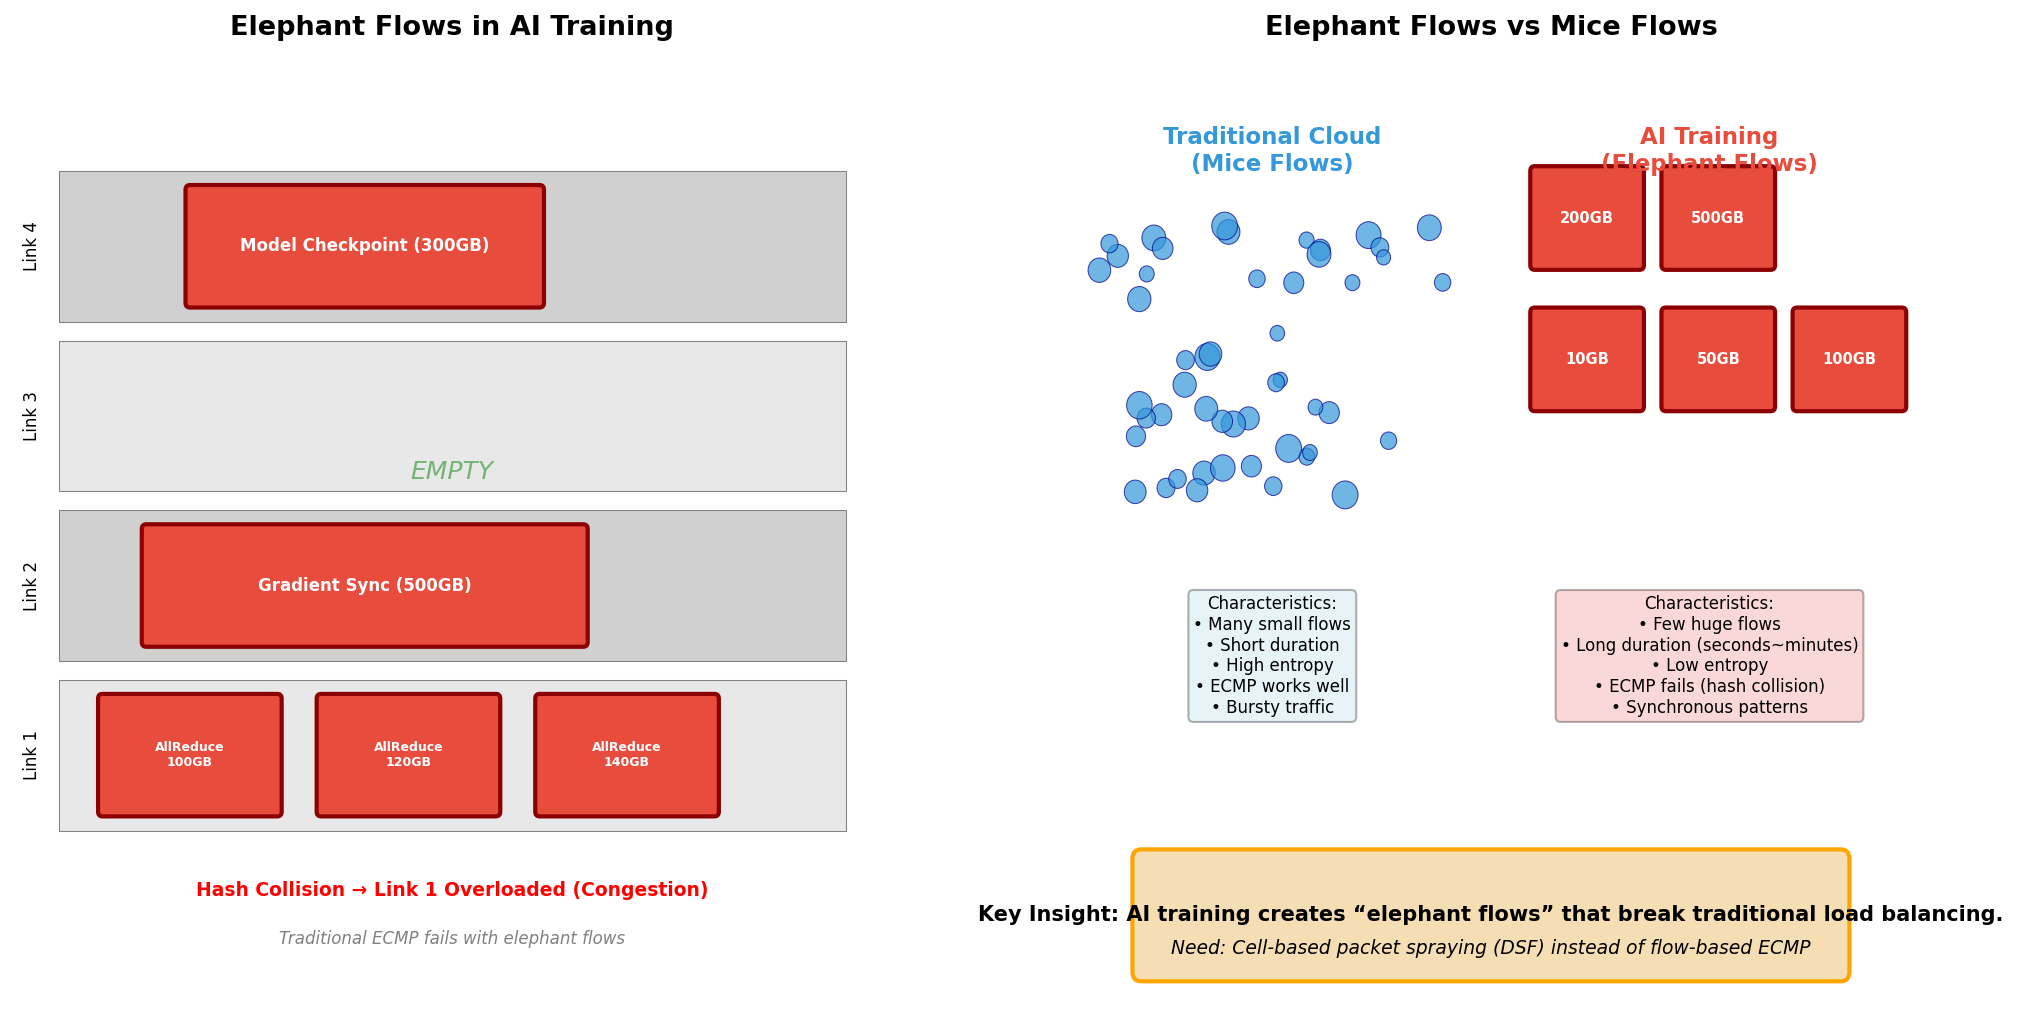
\includegraphics[width=0.9\textwidth]{assets/重构配图/ch06/fig5_elephant_vs_mice_flows.png}
    \caption{大象流与老鼠流对比：AI训练产生少量但巨大的数据流，与传统云计算的小流模式形成对比}
    \label{fig:elephant-vs-mice}
\end{figure}

想象一下高速公路上的交通场景：传统云计算就像繁忙的城市道路，有成千上万的小汽车（小数据包）在各个出口进出；而AI训练则像是在这条公路上行驶超长货车队——绵延数公里的重型卡车编队（大象流）同时出发、同时到达。传统的随机车道分配策略会导致多条超长车队挤在同一条车道，造成严重拥堵，而其他车道却空空如也。

\subsubsection{Insight：为什么ECMP失效了？}

传统的负载均衡机制\textbf{ECMP（Equal-Cost Multi-Path，等价多路径）}依赖哈希算法将流量分散到多条等价路径。其核心假设是：流量足够分散、流数量足够多，哈希结果会自然均衡。

但在AI训练场景中，这两个假设都被打破了：

\begin{enumerate}
    \item \textbf{哈希碰撞}：当只有几十个IP流（低熵）却要分散到数百条链路时，哈希冲突概率急剧上升。多个大象流可能被分配到同一条链路，造成严重的负载不均衡。
    
    \item \textbf{持续时间过长}：大象流一旦开始传输，会持续占用链路带宽数秒甚至数分钟。在ECMP的静态哈希策略下，这种拥塞无法自动缓解。
\end{enumerate}

Meta工程团队最初尝试了多种补救措施：

\begin{itemize}
    \item \textbf{BGP固定路由}：使从加速器经由叶交换机接收的流量根据目的地固定到特定上行链路。这种方法在稳定状态下缓解了低熵问题，但故障场景下失效。
    
    \item \textbf{负载感知ECMP}：能够处理胖流和低熵问题，但调参困难且会产生乱序包——这对RDMA通信是致命的。
    
    \item \textbf{流量工程}：预先计算特定模型使用的流模式，在作业开始前配置叶交换机。但随着网络规模增长，这种方法过于复杂，且其中央化特性使其对故障的响应迟缓。
\end{itemize}

这些尝试揭示了一个深刻洞察：\textbf{修补传统架构无法从根本上解决问题，必须采用全新的设计理念}。

\subsubsection{Design：专用AI网络架构的诞生}

2023年，Meta做出了关键决策：构建专门针对AI工作负载优化的网络架构。这一架构的核心思想是将网络从"通用数据包转发系统"转变为"针对AI优化的数据调度系统"。

专用AI网络的关键特征包括：

\begin{enumerate}
    \item \textbf{细粒度负载均衡}：以数据包或cell为单位进行喷洒，而非以流为单位
    \item \textbf{无哈希转发}：避免低熵流量导致的哈希碰撞问题
    \item \textbf{无损传输}：支持RDMA操作所需的lossless网络
    \item \textbf{可扩展架构}：支持数万GPU的互联
\end{enumerate}

这些需求催生了两大核心技术：\textbf{解耦式调度网络（DSF）}和\textbf{后端聚合（BAG）}。两者的关系可以类比为城市基础设施：DSF是城市内部的道路网络，负责高效地将车辆从起点送达目的地；BAG则是连接多个城市的高速铁路，负责跨区域的快速运输。

\subsection{公有云上的AI超算：AWS EFA详解}

\subsubsection{Problem：公有云能跑超算吗？}

2022年初，亚马逊云科技（AWS）的HPC团队负责人Rahul面对一个棘手的问题。一位来自制药行业的客户正在AWS上运行分子动力学模拟，但遇到了严重的性能瓶颈。

\begin{quote}
"我们在AWS上部署了512个GPU实例，但AllReduce操作的延迟比预期高了一个数量级。同样的代码在本地InfiniBand集群上运行得很好，为什么到了云上就不行了？"
\end{quote}

这是一个具有挑战性的问题。AWS作为全球领先的公有云平台，其网络架构是为通用云计算设计的——强调多租户隔离、灵活性和成本效率，而非极致的HPC性能。传统的TCP/IP协议栈和虚拟化开销使得云网络延迟通常在毫秒级，而HPC应用需要的则是微秒级。

AWS团队尝试了多种方案来优化现有架构：

\begin{itemize}
    \item \textbf{增强ENA（Elastic Network Adapter）}：虽然ENA提供了不错的网络性能，但它仍然基于传统TCP/IP协议栈，无法绕过操作系统内核
    \item \textbf{RoCE v2 over VPC}：尝试在现有以太网基础设施上支持RDMA，但多租户环境下的拥塞控制问题难以解决
    \item \textbf{专用InfiniBand集群}：为特定客户部署专用IB网络，但这违背了公有云的"弹性"和"按需付费"核心理念
\end{itemize}

这些方案要么性能不达标，要么失去了公有云的核心优势。Rahul团队意识到，\textbf{要在公有云上支持超算级AI训练，需要一种全新的网络技术}——它必须同时满足：

\begin{enumerate}
    \item 提供接近InfiniBand的低延迟和高带宽
    \item 在标准以太网基础设施上运行（避免专用硬件成本）
    \item 支持多租户环境的安全隔离
    \item 保持AWS的弹性和按需付费特性
\end{enumerate}

\subsubsection{Insight：SRD的诞生}

经过两年的秘密研发，AWS团队提出了一个创新的解决方案：\textbf{Scalable Reliable Datagram（可扩展可靠数据报，SRD）}协议。

SRD的核心洞察来自于对传统HPC网络的反思。InfiniBand虽然性能卓越，但它依赖专用硬件、采用静态路由、有序传输，这在弹性云环境中显得过于僵化。TCP虽然灵活，但协议栈开销太大。

AWS的解决方案是：\textbf{在标准以太网上构建一个专为云优化的传输协议}。

\begin{insightbox}{SRD的四大设计原则}
\begin{enumerate}
    \item \textbf{智能多路径}：不依赖ECMP哈希，主动将数据喷洒到多条路径
    \item \textbf{无序传输}：允许数据包乱序到达，消除队头阻塞
    \item \textbf{主动拥塞控制}：预防性控制而非反应式控制，保持交换机队列最小
    \item \textbf{硬件卸载}：核心逻辑在Nitro卡硬件中实现，避免操作系统干扰
\end{enumerate}
\end{insightbox}

\subsubsection{Design：EFA+SRD技术实现}

\textbf{1. EFA设备架构}

Elastic Fabric Adapter（EFA）是AWS Nitro系统的一部分，它以一个独立的PCIe设备形式呈现给EC2实例：

\begin{lstlisting}[language=bash,caption=EFA设备识别]
$ lspci | grep -i fabric
00:06.0 Ethernet controller: Amazon.com, Inc. Elastic Fabric Adapter (EFA)
\end{lstlisting}

与ENA不同，EFA设备提供：
\begin{itemize}
    \item \textbf{OS-bypass能力}：应用通过Libfabric API直接与硬件通信，绕过操作系统内核
    \item \textbf{RDMA语义支持}：支持标准的RDMA Verbs接口，兼容现有HPC/AI应用
    \item \textbf{SRD传输层}：底层使用SRD协议替代TCP/UDP
\end{itemize}

\begin{figure}[htbp]
    \centering
    \includegraphics[width=0.95\textwidth]{assets/重构配图/ch06/fig9_efa_architecture.png}
    \caption{AWS EFA架构：Nitro卡上的专用硬件实现SRD协议，提供OS-bypass能力}
    \label{fig:efa-architecture}
\end{figure}

\textbf{2. SRD协议详解}

SRD的技术架构建立在四个核心支柱之上：

\textbf{智能多路径机制}：SRD采用包喷洒策略，可以从数百甚至数千条可用路径中动态选择最多64条并行路径进行单逻辑流的分布式传输。这超越了传统ECMP静态负载均衡的概念。

\begin{itemize}
    \item \textbf{动态路径选择}：持续监控每条路径的RTT，感知拥塞状况
    \item \textbf{亚毫秒级检测切换}：从"较慢"路径动态迁移到"较快"路径
    \item \textbf{ECMP影响}：通过操作封装字段（如UDP源端口号）影响ECMP交换机决策
\end{itemize}

\textbf{可靠性保证}：尽管SRD允许乱序到达，但在可靠性上绝不妥协：

\begin{itemize}
    \item \textbf{亚毫秒重传}：使用Nitro硬件避免操作系统调度延迟，实现亚毫秒级包重传
    \item \textbf{路径多样化重传}：重传包选择不同路径，提高重传成功率
    \item \textbf{并行未完成消息}：允许网络上存在多个未完成消息，提高链路利用率
\end{itemize}

\textbf{主动拥塞控制}：SRD采用"预防胜于治疗"的设计理念：

\begin{figure}[htbp]
    \centering
    \includegraphics[width=0.95\textwidth]{assets/重构配图/ch06/fig10_srd_congestion_control.png}
    \caption{SRD拥塞控制流程：动态路径选择与主动拥塞避免机制}
    \label{fig:srd-congestion-control}
\end{figure}

核心目标是保持交换机队列长度在最小水平，避免队列膨胀导致的延迟增加。SRD结合动态速率限制和精确的在途包量控制，持续估算可用带宽和RTT，主动降低传输速率。

\textbf{3. EFA-only接口}

2024年10月，AWS发布了EFA-only接口类型，解除了EFA与ENA的耦合：

\begin{table}[htbp]
\centering
\caption{EFA接口类型对比}
\begin{tabular}{lcc}
\toprule
\textbf{特性} & \textbf{EFA + ENA} & \textbf{EFA-only} \\
\midrule
IP地址 & 需要（每个接口一个） & 不需要 \\
最大接口数 & 受限于IP地址空间 & 更多 \\
主要用途 & HPC/ML混合工作负载 & 纯AI训练集群 \\
Linux路由问题 & 可能存在源IP不匹配 & 无 \\
\bottomrule
\end{tabular}
\end{table}

EFA-only接口使用MAC地址而非IP地址进行通信，解决了大规模集群中的IP地址耗尽和Linux多接口路由问题。

\subsubsection{Comparison：SRD vs InfiniBand}

SRD与InfiniBand在设计哲学上存在显著差异：

\begin{table}[htbp]
\centering
\caption{AWS SRD与InfiniBand技术对比}
\begin{tabular}{lcc}
\toprule
\textbf{特性} & \textbf{AWS SRD (EFA)} & \textbf{InfiniBand} \\
\midrule
传输模型 & 消息（无序） & 消息（有序） \\
路径选择 & ECMP喷洒+动态负载均衡 & 单一路径（自适应路由） \\
重传超时 & 动态估算（微秒级） & 静态配置（对数刻度） \\
拥塞控制 & 动态速率限制 & 静态速率限制 \\
硬件依赖 & Nitro专用DPU & 专用IB交换机和网卡 \\
部署灵活性 & 标准以太网交换机 & 专用IB网络 \\
云原生支持 & 原生支持多租户 & 需专用网络分区 \\
\bottomrule
\end{tabular}
\end{table}

\begin{insightbox}{SRD与InfiniBand的选择逻辑}
\begin{itemize}
    \item \textbf{选择SRD}：需要云弹性、多租户共享、快速扩缩容的AI训练场景
    \item \textbf{选择InfiniBand}：追求极致延迟（<2μs）、确定性性能、专用集群的HPC场景
\end{itemize}
\end{insightbox}

\subsection{云厂商AI网络技术路线对比}

\subsubsection{三种不同的技术哲学}

在AI训练网络领域，Meta、AWS和Google代表了三种截然不同的技术哲学：

\begin{enumerate}
    \item \textbf{Meta：开放解耦哲学}
    
    Meta的DSF架构体现了"解耦一切"的设计理念。通过OCP-SAI（开放计算项目交换机抽象接口）和FBOSS（Facebook开放交换机系统），Meta实现了：
    
    \begin{itemize}
        \item 交换机硬件与软件的解耦
        \item 线卡与交换网板的解耦
        \item 网络设备与终端NIC的解耦
    \end{itemize}
    
    这种哲学的优势在于灵活性和供应商多样性。DSF支持来自NVIDIA、AMD、Broadcom和Meta自研MTIA的各种加速器。
    
    \item \textbf{AWS：云原生创新哲学}
    
    AWS选择了一条不同的道路：在标准以太网基础设施上，通过专有协议和硬件创新实现超算性能。其核心是Nitro系统——AWS自研的DPU家族。
    
    SRD协议完全运行在Nitro硬件中，带来了独特的护城河优势。使用现成设备的数据中心无法直接复制这种架构，必须等待市场推出类似的硬件实现。
    
    这种哲学的优势在于能够在公有云的多租户环境中提供一致的高性能。
    
    \item \textbf{Google：垂直整合哲学}
    
    Google的AI网络策略是与TPU芯片紧密集成的。从TPU v2开始，Google就为每代TPU设计了专用的Inter-Chip Interconnect（ICI）。
    
    更令人瞩目的是Google在TPU v4中引入的光电路交换机（OCS），通过机械镜阵列动态重构光路连接，实现了物理拓扑的灵活重组。
    
    这种哲学的优势在于全栈优化——从芯片到交换机，每一层都为AI工作负载量身定制。
\end{enumerate}

\subsubsection{技术路线对比}

\begin{table}[htbp]
\centering
\caption{云厂商AI网络技术路线对比}
\begin{tabular}{p{2.5cm}p{3.5cm}p{3.5cm}p{3.5cm}}
\toprule
\textbf{维度} & \textbf{Meta DSF} & \textbf{AWS EFA} & \textbf{Google TPU} \\
\midrule
核心架构 & 解耦式调度网络 & Nitro硬件加速+SRD & 3D Torus+OCS \\
拓扑类型 & Clos+包喷洒 & 标准VPC网络 & 3D环面拓扑 \\
传输协议 & RoCE v2 & 专有SRD & 专有ICI \\
扩展能力 & 18K+ GPU & 数千GPU & 8,960 TPU \\
负载均衡 & Cell级包喷洒 & Packet spraying & 拓扑感知路由 \\
拥塞控制 & VOQ+信用机制 & 主动拥塞控制 & 端到端流量控制 \\
技术哲学 & 开放标准+自研 & 专有协议+硬件 & 全栈垂直整合 \\
适用场景 & 大规模自建集群 & 公有云AI训练 & TPU专属工作负载 \\
\bottomrule
\end{tabular}
\end{table}

\subsubsection{OSI模型视角下的技术栈对比}

从网络协议栈的分层视角，三大厂商的技术选择差异更加清晰：

\begin{table}[htbp]
\centering
\caption{云厂商数据中心网络技术栈对比}
\begin{tabular}{lccc}
\toprule
\textbf{OSI层} & \textbf{AWS} & \textbf{Google Cloud} & \textbf{Microsoft Azure} \\
\midrule
L7应用层 & EFA API & Cloud RDMA API & InfiniBand Verbs API \\
L6表示层 & Nitro内部编码 & ALTS内部加密 & Azure Boost编码 \\
L5会话层 & Nitro会话管理 & 内部RPC (gRPC) & MANA会话管理 \\
L4传输层 & SRD & Falcon & RoCE v2 + InfiniBand \\
L3网络层 & VPC + ENA Express & Andromeda 2.1 & AccelNet/MANA \\
L2数据链路层 & Ethernet & Ethernet & Ethernet/InfiniBand \\
L1物理层 & QSFP-DD + PAM4 & 标准光纤+OCS & 标准光纤+PAM4/HCF \\
\midrule
硬件加速单元 & Nitro v5 DPU & Intel IPU E2000 & Azure Boost + MANA \\
\bottomrule
\end{tabular}
\end{table}

\subsection{公有云AI训练实践与挑战}

\subsubsection{Challenge：多租户环境下的网络保障}

公有云的核心特征是多租户共享。对于AI训练这种对网络延迟和带宽极其敏感的工作负载，多租户带来了一系列独特挑战：

\textbf{1. 邻居效应（Noisy Neighbor）}

在共享网络基础设施中，一个租户的大象流可能会影响其他租户的性能。AWS EFA通过SRD的多路径能力来缓解这一问题：

\begin{itemize}
    \item 当某条路径出现拥塞时，SRD自动切换到其他路径
    \item 不同租户的流量天然分布在不同路径上
    \item 即使发生路径冲突，亚毫秒级的路径切换也能将干扰降至最低
\end{itemize}

\textbf{2. 虚拟化开销}

传统虚拟化网络需要经过hypervisor、虚拟交换机等多个软件层，带来显著延迟。三大云厂商的解决方案：

\begin{itemize}
    \item \textbf{AWS}：Nitro系统通过专用硬件处理网络虚拟化，主机CPU零参与
    \item \textbf{Azure}：MANA（Microsoft Azure Network Adapter）提供类似SR-IOV的硬件直通能力
    \item \textbf{Google}：IPU（Infrastructure Processing Unit）将网络功能卸载到专用芯片
\end{itemize}

\subsubsection{权衡：成本与性能}

公有云AI训练需要在成本和性能之间做出权衡：

\textbf{1. 网络方案选择}

\begin{table}[htbp]
\centering
\caption{公有云AI训练网络方案成本对比（估算）}
\begin{tabular}{lccc}
\toprule
\textbf{方案} & \textbf{相对成本} & \textbf{适用规模} & \textbf{最佳场景} \\
\midrule
标准ENA/TCP & 1x & 单节点/小集群 & 推理、小规模训练 \\
EFA-only & 1.2x & 中等规模集群 & 多数AI训练工作负载 \\
EFA+ENA混合 & 1.3x & 混合工作负载 & 同时需要HPC和常规网络 \\
专用InfiniBand & 2x+ & 大规模专用集群 & 追求极致性能的HPC \\
\bottomrule
\end{tabular}
\end{table}

\textbf{2. 弹性vs专用}

\begin{itemize}
    \item \textbf{按需实例}：适合实验性开发和训练任务，EFA可以随实例自动启用
    \item \textbf{预留实例/Spot}：长期训练任务可显著降低成本，EFA同样适用
    \item \textbf{专用集群}：对延迟极度敏感的场景可考虑，但失去了云的核心优势
\end{itemize}

\subsubsection{最佳实践建议}

基于公有云AI训练的实践经验，我们总结以下建议：

\begin{insightbox}{公有云AI训练网络优化建议}
\begin{enumerate}
    \item \textbf{选择合适的实例类型}：P5/P5en实例标配EFA，适合大规模分布式训练
    \item \textbf{启用EFA-only接口}：大规模集群时使用，避免IP地址限制
    \item \textbf{使用Placement Group}：将实例部署在物理位置相近的可用区，降低网络延迟
    \item \textbf{监控SRD性能指标}：利用CloudWatch监控SRD重传率、路径利用率等指标
    \item \textbf{合理规划网络拓扑}：对于超大规模训练，考虑使用BAG类似的跨区域互联方案
\end{enumerate}
\end{insightbox}

\subsection{Prometheus项目：构建吉瓦级AI集群的挑战}

\subsubsection{Problem：万卡集群的互联难题}

2024年初，Meta启动了代号"Prometheus"的雄心勃勃的项目：构建一个1吉瓦（Gigawatt）级别的AI训练集群，横跨五个数据中心建筑，互联数万GPU。这是Meta历史上最大的单体基础设施项目。

项目负责人Sarah面临着一个看似不可能完成的任务：

\begin{quote}
"我们需要把分布在多个数据中心建筑中的GPU互联成一个统一的计算池。但数据中心之间的距离意味着光纤长度可能达到数十公里，如何在保持性能的同时实现这种超大规模互联？"
\end{quote}

传统方案是在每个数据中心部署独立的AI集群，通过上层网络互联。但这会带来两个问题：

\begin{enumerate}
    \item \textbf{性能瓶颈}：跨区域通信需要经过多层网络，延迟和带宽都无法满足AI训练的需求
    \item \textbf{资源碎片化}：每个集群独立调度，无法实现全局优化
\end{enumerate}

\subsubsection{Insight：为什么需要超级脊层？}

Sarah和她的团队意识到，解决这个问题的关键在于引入一个新的网络层——\textbf{超级脊层（Super Spine）}，专门负责跨区域的高速互联。这就是\textbf{后端聚合（BAG）}技术的核心思想。

\begin{insightbox}{BAG的核心设计思想}
BAG作为区域网络与Meta骨干网之间的聚合点，采用集中式超级脊层连接多个L2网络结构。这种设计将分布式计算资源通过高容量网络抽象为统一的计算池。
\end{insightbox}

关键洞察在于：\textbf{跨区域互联不应该"借用"通用网络，而应该构建专用的AI后端网络}。BAG作为一个独立的网络层，可以针对AI工作负载的特性进行专门优化，而不受通用网络设计约束。

\subsubsection{Design：BAG架构详解}

\begin{figure}[htbp]
    \centering
    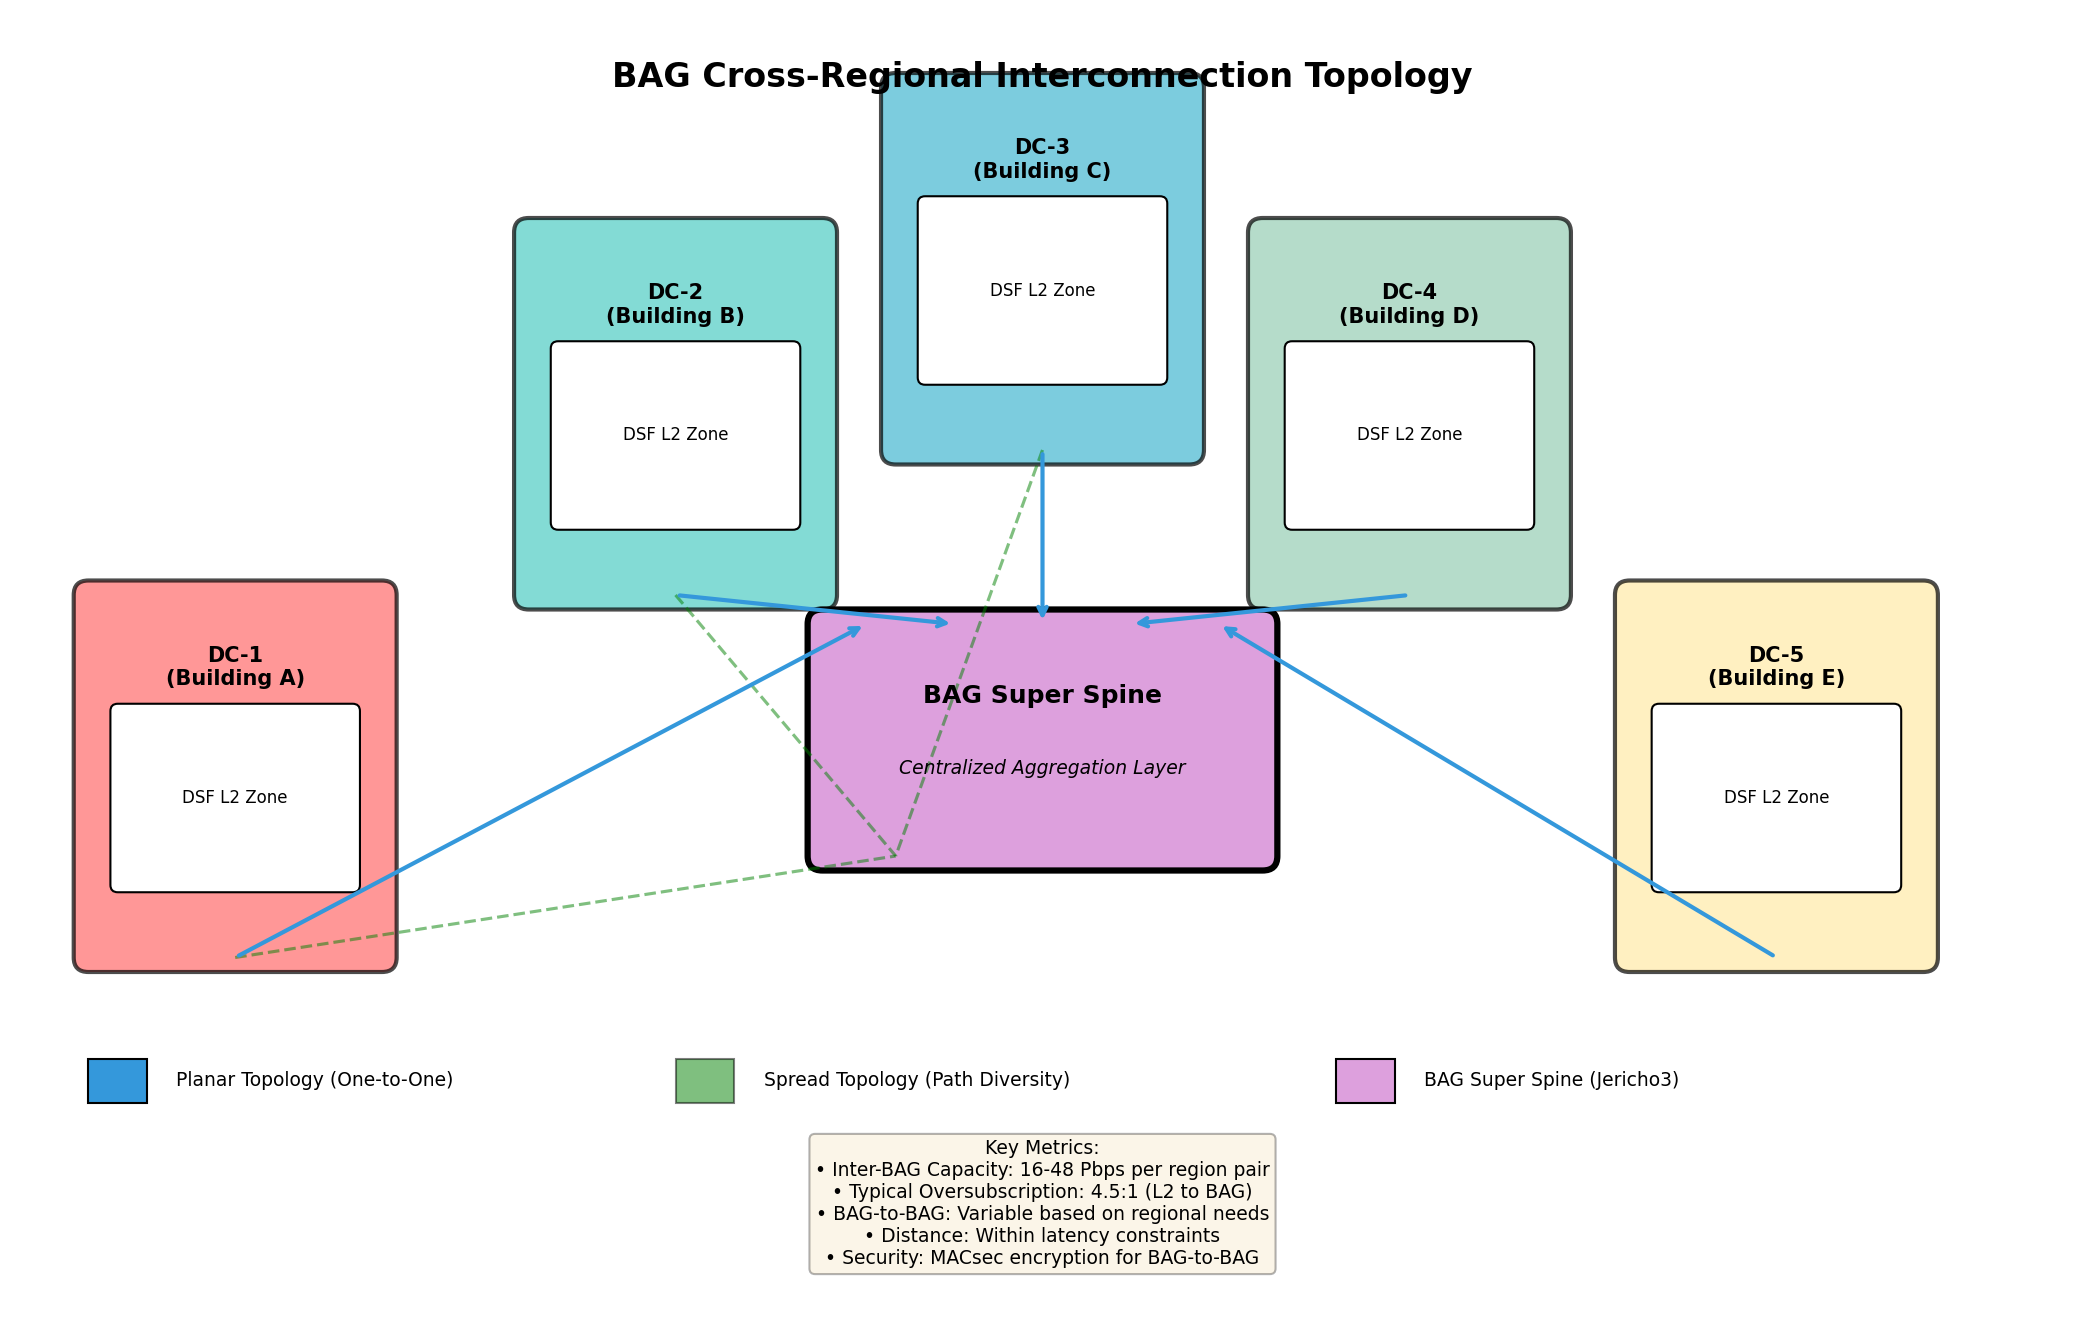
\includegraphics[width=0.95\textwidth]{assets/重构配图/ch06/fig2_bag_topology.png}
    \caption{BAG跨区域互联拓扑：五个数据中心通过BAG超级脊层互联，支持平面和分散两种连接拓扑}
    \label{fig:bag-topology}
\end{figure}

BAG架构的设计体现了工程上的深思熟虑：

\textbf{1. 硬件选择}

BAG采用配备Jericho3（J3）ASIC线卡的机箱式交换机，每块线卡提供多达432个800G端口。这种高密度配置使BAG能够以PB级带宽（例如每对区域之间16-48 Pbps）支持区域间的海量数据传输。

为什么选择Jericho3？关键原因是\textbf{深缓冲区（Deep Buffer）}能力。由于BAG-to-BAG连接跨越较长物理距离，需要深缓冲区来支持如PFC（基于优先级的流控制）等无损拥塞控制协议。深缓冲区提供了充足的头部空间（headroom buffer），确保在网络拥塞时不会丢失数据包——这对RDMA通信至关重要。

\textbf{2. 拓扑选择}

BAG层在区域间支持两种连接拓扑：

\begin{itemize}
    \item \textbf{平面拓扑（Planar）}：BAG交换机按照平面一对一连接，管理相对简单但将潜在的故障域集中
    \item \textbf{分散拓扑（Spread）}：链路分布在多个BAG交换机和平面上，增强了路径多样性和系统韧性
\end{itemize}

拓扑选择依据主要是站点规模和光纤可用性。对于Prometheus这种超大规模部署，分散拓扑提供了更好的故障隔离能力。

\textbf{3. 超配策略}

从L2结构到BAG的典型超配比约为\textbf{4.5:1}。这是一种成本与性能的权衡：并非所有GPU都需要同时以满带宽与其他区域的GPU通信，因此可以适当减少上行带宽以降低成本。

\subsubsection{Proof：Prometheus的实战经验}

Prometheus项目的部署验证了BAG架构的可行性：

\begin{itemize}
    \item 成功实现了横跨五个数据中心建筑的统一AI集群
    \item 跨区域通信带宽达到设计目标，满足大规模分布式训练需求
    \item 通过分散拓扑和深缓冲区设计，有效应对了光纤距离带来的挑战
\end{itemize}

更重要的是，BAG架构为未来扩展奠定了基础。Meta已经宣布了规模更大的Hyperion项目（预计2028年上线，容量达5吉瓦），BAG的模块化设计使其能够平滑扩展以支持更大规模的集群。

\subsection{DSF：解耦式调度网络的工程智慧}

\subsubsection{Problem：突破物理交换机的限制}

在构建24,000 GPU集群时，Meta网络工程师Tom遇到了一个物理限制：单体机箱式交换机的端口数量无法满足需求。传统的解决方案是增加网络层级，但这会带来更高的延迟和更复杂的拓扑。

\begin{quote}
"我们需要一种方法，既能突破单机箱的物理限制，又能保持低延迟和高性能。传统的堆叠方案只是权宜之计，不能从根本上解决问题。"
\end{quote}

\subsubsection{Insight：解耦的哲学}

Tom团队从超级计算机的互连技术中获得灵感：\textbf{将线卡和交换网板解耦为独立互联的硬件设备}，构建分布式交换系统。这就是\textbf{解耦式调度网络（Disaggregated Scheduled Fabric, DSF）}的核心思想。

\begin{figure}[htbp]
    \centering
    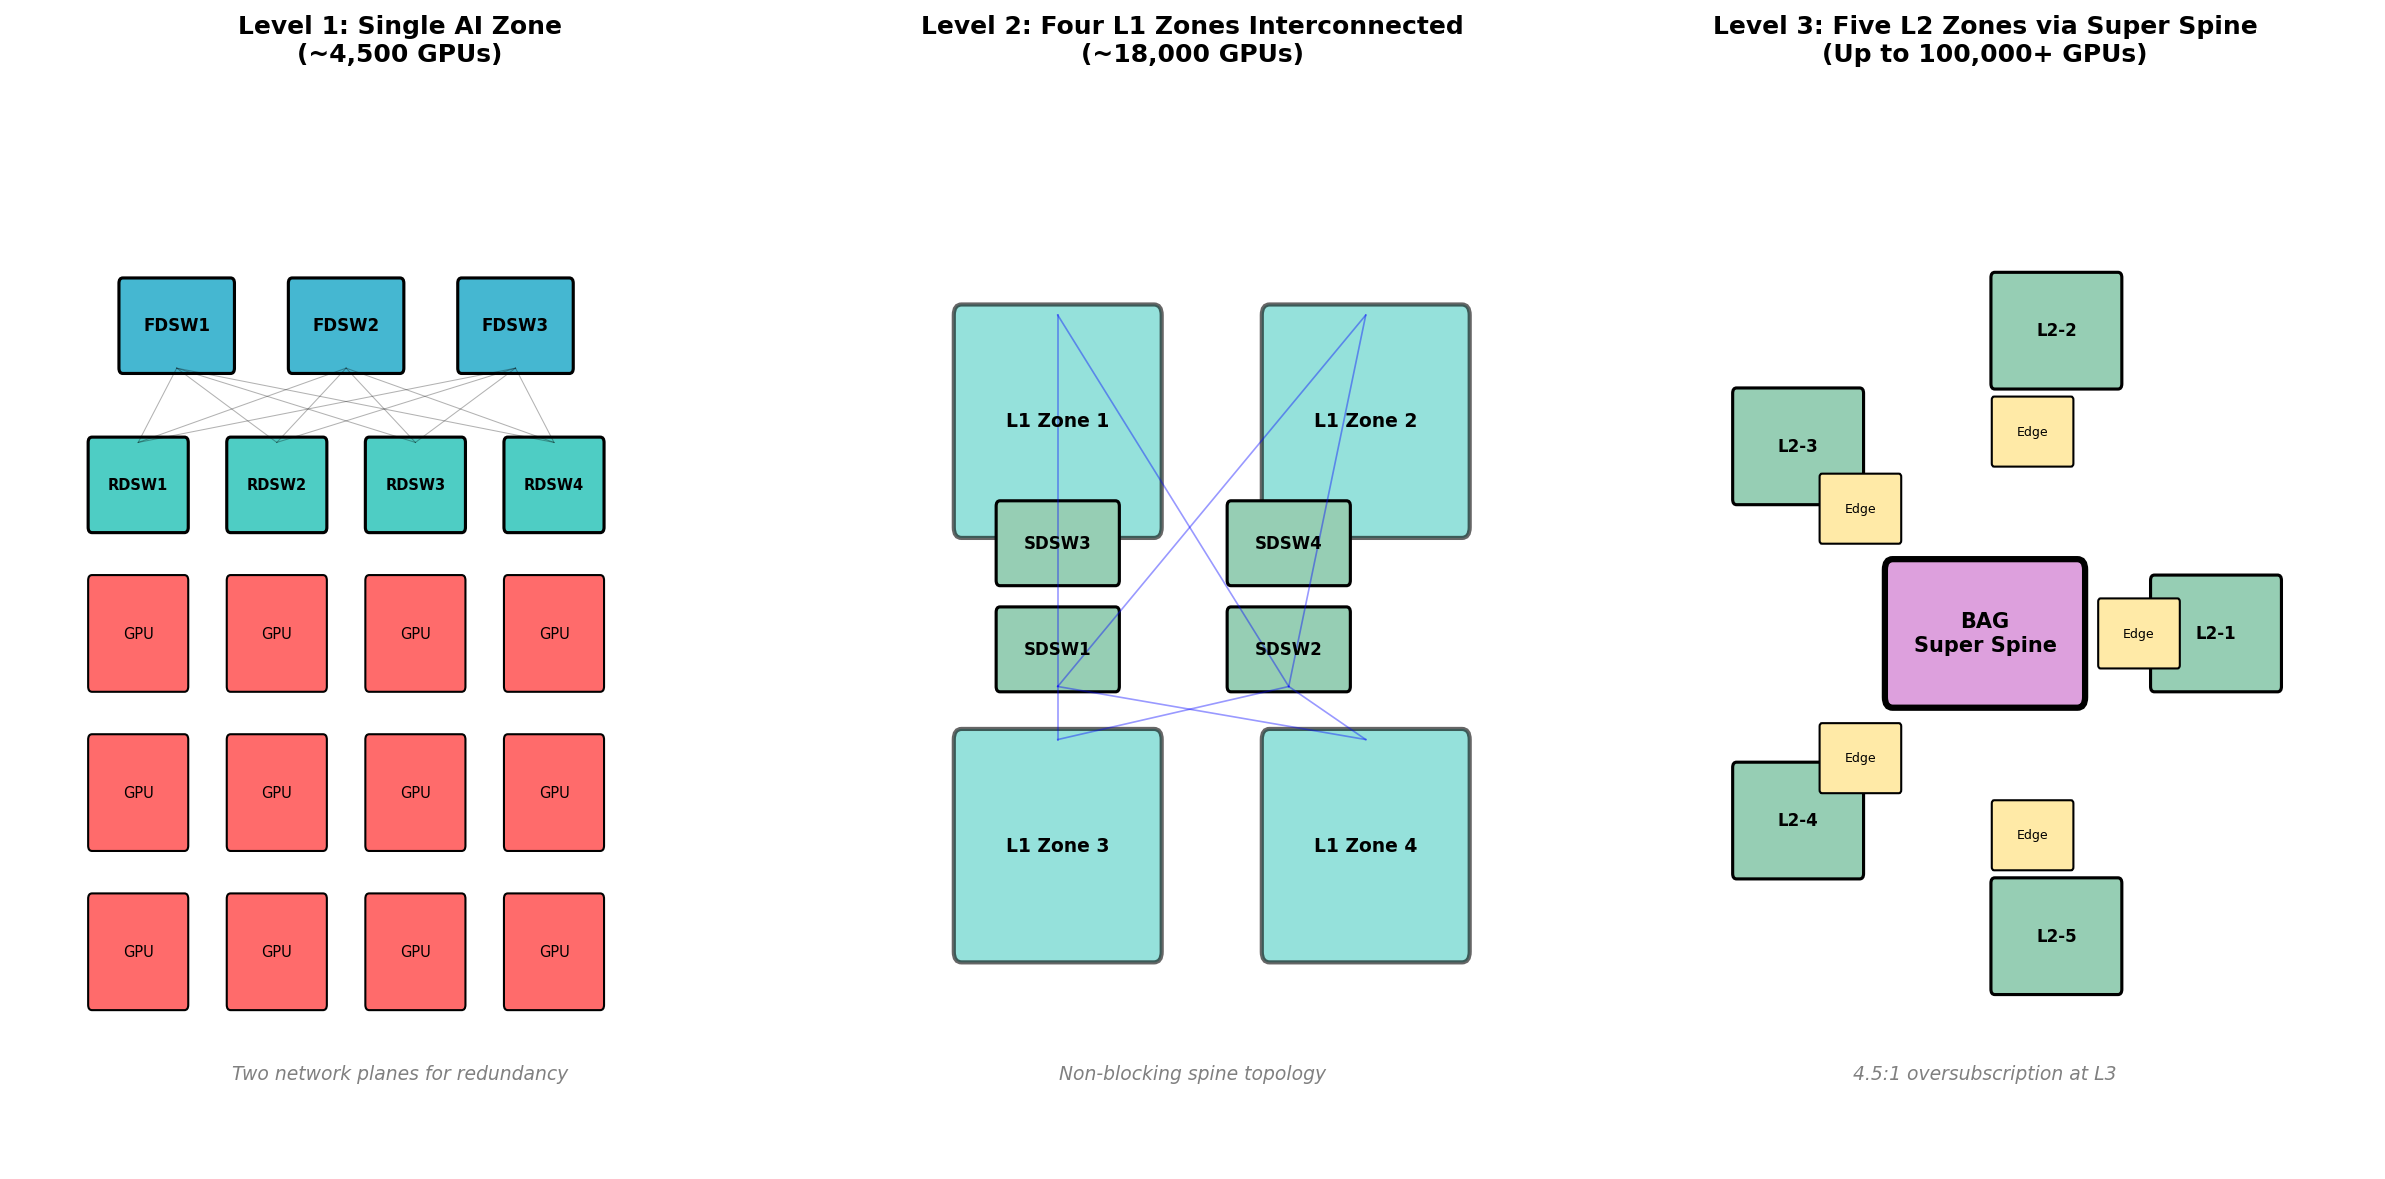
\includegraphics[width=0.95\textwidth]{assets/重构配图/ch06/fig3_dsf_three_tiers.png}
    \caption{DSF三级扩展架构：L1（单AI区域）、L2（四个L1互联）、L3（跨区域BAG互联）}
    \label{fig:dsf-three-tiers}
\end{figure}

DSF的核心洞察是\textbf{双域架构}：

\begin{itemize}
    \item \textbf{以太网域}：负责与传统网络基础设施的交互，处理标准以太网协议
    \item \textbf{交换结构域}：负责高效的数据包单元分发，采用创新的包喷洒技术
\end{itemize}

这种设计就像现代化的邮政系统：以太网域是街道地址系统，交换结构域则是包裹分拣中心。对外部而言，分布式的接口节点和交换节点表现为单一统一的交换机。

\subsubsection{Design：DSF的关键创新}

\textbf{1. 虚拟输出队列（VOQ）}

传统网络使用简单的输入队列，存在\textbf{队头阻塞（Head-of-Line Blocking）}问题——如果队列最前面的数据包被阻塞，后面所有数据包都无法前进。

VOQ机制为\textbf{每个目标端口独立维护虚拟队列}。这就像机场为每个目的地航班设立独立的候机室，每个目的地的乘客在各自的候机室等待，互不影响。当某个输出端口拥塞时，只有指向该端口的流量受到影响，其他流量继续正常传输。

\textbf{2. 包喷洒（Packet Spraying）}

这是DSF最具创新性的特性。与依赖哈希的传统方法不同，DSF在结构域内将数据包分割为单元（cells），\textbf{均匀喷洒在所有可用路径上}，在出接口处重新组装。

这种技术依赖于基于信用的分配机制（credit-based allocation）。入口接口节点动态地向出口接口节点请求信用令牌，系统根据当前路径可用性、拥塞水平和带宽利用率做出实时决策。

\begin{insightbox}{包喷洒 vs ECMP}
\begin{itemize}
    \item ECMP：以流为单位，依赖哈希，存在哈希碰撞风险
    \item 包喷洒：以cell为单位，均匀分布，自动适应负载变化
\end{itemize}
\end{insightbox}

\textbf{3. 三级扩展架构}

DSF通过三级扩展支持不同规模的AI集群：

\begin{enumerate}
    \item \textbf{L1（AI区域）}：包含多个扩展单元，每个单元是一组连接到RDSW的GPU机架。同一区域内的所有RDSW通过公共的FDSW层互联，支持约4,500 GPU。
    
    \item \textbf{L2（二级脊层）}：通过SDSW（二级脊DSF交换机）互连四个DSF L1区域，形成非阻塞拓扑，支持高达18,000 GPU。
    
    \item \textbf{L3（超级脊层）}：通过BAG互联五个DSF L2区域，构建吉瓦级集群，支持100,000+ GPU。
\end{enumerate}

\textbf{4. 输入平衡模式}

DSF引入了\textbf{输入平衡模式}（input-balanced mode），智能地平衡各层之间的可达性信息，确保在发生故障时避免在结构层和脊层出现拥塞。这种前瞻性设计体现了对大规模网络中故障常态化的深刻认识。

\subsubsection{Analysis：DSF的工程价值}

DSF架构的价值体现在多个维度：

\begin{enumerate}
    \item \textbf{性能}：包喷洒技术实现了接近最优的负载均衡，有效利用全部带宽容量
    \item \textbf{可扩展性}：解耦架构突破了物理交换机的限制，支持平滑扩展
    \item \textbf{灵活性}：双域设计允许独立演进，适应未来技术变化
    \item \textbf{可靠性}：VOQ和输入平衡模式提升了系统的故障容忍能力
\end{enumerate}

\subsection{Scale-Up网络的演进趋势：从GTC 2024看未来}

Meta的实践为AI训练网络的发展提供了宝贵的工程经验，但技术的发展永远不会止步。2024年的GTC大会上，NVIDIA展示了一系列突破性进展，揭示了Scale-Up网络正在进入一个全新阶段：从单机柜互联走向跨机柜、异构协同的大规模系统域扩展。

\subsubsection{Insight：Scale-Up域的持续扩展}

GTC 2024释放了一个清晰的信号：\textbf{AI集群中的"高性能通信域"正在被尽量做大}。

\begin{insightbox}{从NVL72到NVL576的跨越}
\begin{itemize}
    \item \textbf{NVL72}：单Rack 72 GPU高带宽互联
    \item \textbf{NVL576}：8个Rack互联形成576 GPU更大Scale-Up域
    \item \textbf{Rubin Ultra}：144 GPU通过NVL backplane连接
\end{itemize}
这种演进的核心思想是：以高密机柜为基础，通过分层多级扩展构建更大规模的Scale-Up域。
\end{insightbox}

这种扩展背后的驱动力是AI模型规模的爆炸式增长。大模型训练中的张量并行、流水并行需要更大的通信域；推理中的Prefill/Decode分离部署也需要更复杂的协同。单Rack的72 GPU已经无法满足需求，必须将多个Rack"拼"成更大的计算池。

\subsubsection{架构路线分化：NVIDIA vs 阿里云UPN}

有趣的是，业界对于"如何做大Scale-Up域"出现了两种截然不同的设计哲学。

\textbf{1. NVIDIA路线：分层多级扩展}

NVIDIA的核心思路可以概括为：\textbf{先做大单Rack Scale-Up，再通过第二级互联将多个Rack组合成更大Scale-Up域}。

\begin{figure}[htbp]
    \centering
    \includegraphics[width=0.95\textwidth]{assets/重构配图/ch06/fig7_nvidia_vs_upn_architecture.mmd}
    \caption{NVIDIA分层多级扩展 vs 阿里云UPN单层大域交换：两种设计哲学的对比}
    \label{fig:nvidia-vs-upn}
\end{figure}

NVL576采用明显的两层结构：
\begin{itemize}
    \item \textbf{第一层}：单Rack内72 GPU高密度互联（NVSwitch L1）
    \item \textbf{第二层}：8个Rack之间通过NVSwitch L2互联
\end{itemize}

这一路线的优势在于扩展路径自然、工程实现平滑、物理层成本可控（Rack内铜、Rack间光）。但其代价是分层拓扑引入的\textbf{带宽非均匀性}——Rack内通信带宽显著高于跨Rack通信。

\textbf{2. 阿里云UPN路线：单层大域交换}

与NVIDIA相比，阿里云UPN体现的是另一类设计哲学：\textbf{尽可能在统一交换层中构建更大、带宽更均匀的Scale-Up域}。

UPN的典型特征是：
\begin{itemize}
    \item 单层switch互联，所有流量经过同一级交换转发
    \item 网络带宽更均匀，拓扑语义更简单
    \item 更适合复杂通信模式（如MoE中的all-to-all）
\end{itemize}

当前一代UPN支持512 GPU，下一代将扩展到576甚至1152 GPU。更重要的是，UPN实现了\textbf{高密系统解耦}——计算节点形态与互联层可以更灵活分离。

\subsubsection{物理层分层设计：铜与光的协作}

GTC 2024展示的另一个重要趋势是物理层的分层设计。大规模Scale-Up网络在物理层走向"近端铜、远端光"的分层策略：

\begin{figure}[htbp]
    \centering
    \includegraphics[width=0.95\textwidth]{assets/重构配图/ch06/fig8_physical_layer_hierarchy.mmd}
    \caption{Scale-Up网络物理层分层设计：Rack内铜互联与Rack间光互联的协作}
    \label{fig:physical-layer-hierarchy}
\end{figure}

\begin{table}[htbp]
\centering
\caption{铜互联 vs 光互联在Scale-Up网络中的适用场景}
\begin{tabular}{lcc}
\toprule
\textbf{特性} & \textbf{Rack内（铜）} & \textbf{Rack间（光）} \\
\midrule
距离 & \textless 1m & 1-10m+ \\
成本 & 低 & 高 \\
功耗 & 低 & 较高 \\
信号完整性 & 优秀 & 良好 \\
布线复杂度 & 简单 & 可管理 \\
速率升级路径 & 受限 & 灵活 \\
\bottomrule
\end{tabular}
\end{table}

这种分层设计的本质是在\textbf{逻辑上保持统一高性能互联}，在\textbf{物理上做成本/性能最优选择}。它不是技术上的妥协，而是工程智慧的体现。

\subsubsection{异构协同：GPU与专用推理芯片的互联}

GTC 2024还展示了一个令人兴奋的趋势：\textbf{异构节点通过低时延网络协同工作}。

NVIDIA展示了Rubin NVL72与Groq 3 LPX Rack的协同使用场景：
\begin{itemize}
    \item \textbf{GPU Rack}：负责高算力、长上下文、高吞吐的Prefill
    \item \textbf{LPU Rack}：负责低时延、高token rate的Decode
    \item \textbf{互联方式}：通过NIC + 以太网特殊低时延模式进行ping-pong式交互
\end{itemize}

这意味着未来AI系统的结构将演化为：不同Rack负责不同计算负载，系统整体规模远大于单一计算节点集群。\textbf{Scale-Up与Scale-Out的边界正在模糊}——Rack内部继续极致化高带宽Scale-Up，Rack之间则通过低时延Ethernet/InfiniBand形成系统级协同。

\subsubsection{核心挑战的转变}

随着Scale-Up从单机柜走向多Rack、异构协同和更大系统域，挑战已经不再只是"带宽够不够"，而是一个涉及网络架构、系统软件、运维体系的综合问题。

\begin{insightbox}{Scale-Up网络竞争焦点的转移}
\begin{enumerate}
    \item 从"峰值带宽"转向"系统稳定性"
    \item 从"理论性能"转向"尾时延控制"
    \item 从"封闭专有"转向"开放运维生态"
\end{enumerate}
\end{insightbox}

Meta在其DSF架构中采用的开放网络操作系统（SONiC）思路，正是这种转变的体现。当AI集群进入大规模生产阶段，真正决定TCO的不是"理论带宽"，而是\textbf{稳定性、可维护性与故障恢复效率}。

\begin{figure}[htbp]
    \centering
    \includegraphics[width=0.95\textwidth]{assets/重构配图/ch06/fig6_scaleup_evolution_timeline.mmd}
    \caption{Scale-Up网络演进时间线：从NVLink 1.0到Rubin Ultra的技术跃迁}
    \label{fig:scaleup-evolution}
\end{figure}

\subsubsection{对Meta实践的启示}

GTC 2024展示的行业趋势为Meta的DSF和BAG架构提供了重要验证，同时也揭示了未来演进方向：

\begin{enumerate}
    \item \textbf{Scale-Up域继续做大是行业共识}：Meta的BAG架构提前布局了跨区域超级脊层，与NVL576的扩展思路不谋而合。
    
    \item \textbf{分层设计是工程现实}：Meta在DSF中采用的"Rack内密集互联+Rack间光互联"策略，与NVIDIA的"铜+光"分层完全一致。
    
    \item \textbf{开放生态将成为关键变量}：Meta采用SONiC作为开放网络操作系统，使其能够复用数据中心级的运维能力。随着规模扩大，这一点将越来越重要。
    
    \item \textbf{异构协同是下一阶段重点}：Meta已经开始探索GPU与专用芯片的协同，未来可能需要支持更复杂的异构计算场景。
\end{enumerate}

\subsection{当AI训练卡住时：调试工具的诞生}

\subsubsection{Problem：万卡集群的调试噩梦}

2023年中，Meta的一个大型训练作业突然停滞。6,000 GPU集群全部"卡死"，训练进度不再前进。运维工程师David接到告警，面对一个棘手的问题：在6,000个GPU中，是哪个出了问题？

\begin{quote}
"在传统服务器集群中，单个节点故障不会影响整体。但在AI训练中，所有GPU必须保持同步——一个慢节点会拖慢整个集群。找出这个'掉队者'就像在数万人中找出一个走得稍慢的人。"
\end{quote}

传统调试工具在这种场景下完全失效：

\begin{itemize}
    \item 单个GPU的日志无法反映全局状态
    \item 网络监控无法定位同步问题
    \item 重启训练成本高昂（可能需要数小时重新初始化）
\end{itemize}

\subsubsection{Insight：同步问题的本质}

David团队深入分析了问题本质。AI训练中的集体通信操作（如AllReduce）要求所有参与者在同步点等待彼此。如果某个GPU由于硬件故障、网络抖动或软件问题而变慢，整个集群都会等待。

关键洞察：\textbf{同步问题具有传播性}——一个慢节点的影响会扩散到整个集群。因此，调试工具需要具备分布式视角，能够同时监控所有节点的状态。

\subsubsection{Design：desync debug与Flight Recorder}

\begin{figure}[htbp]
    \centering
    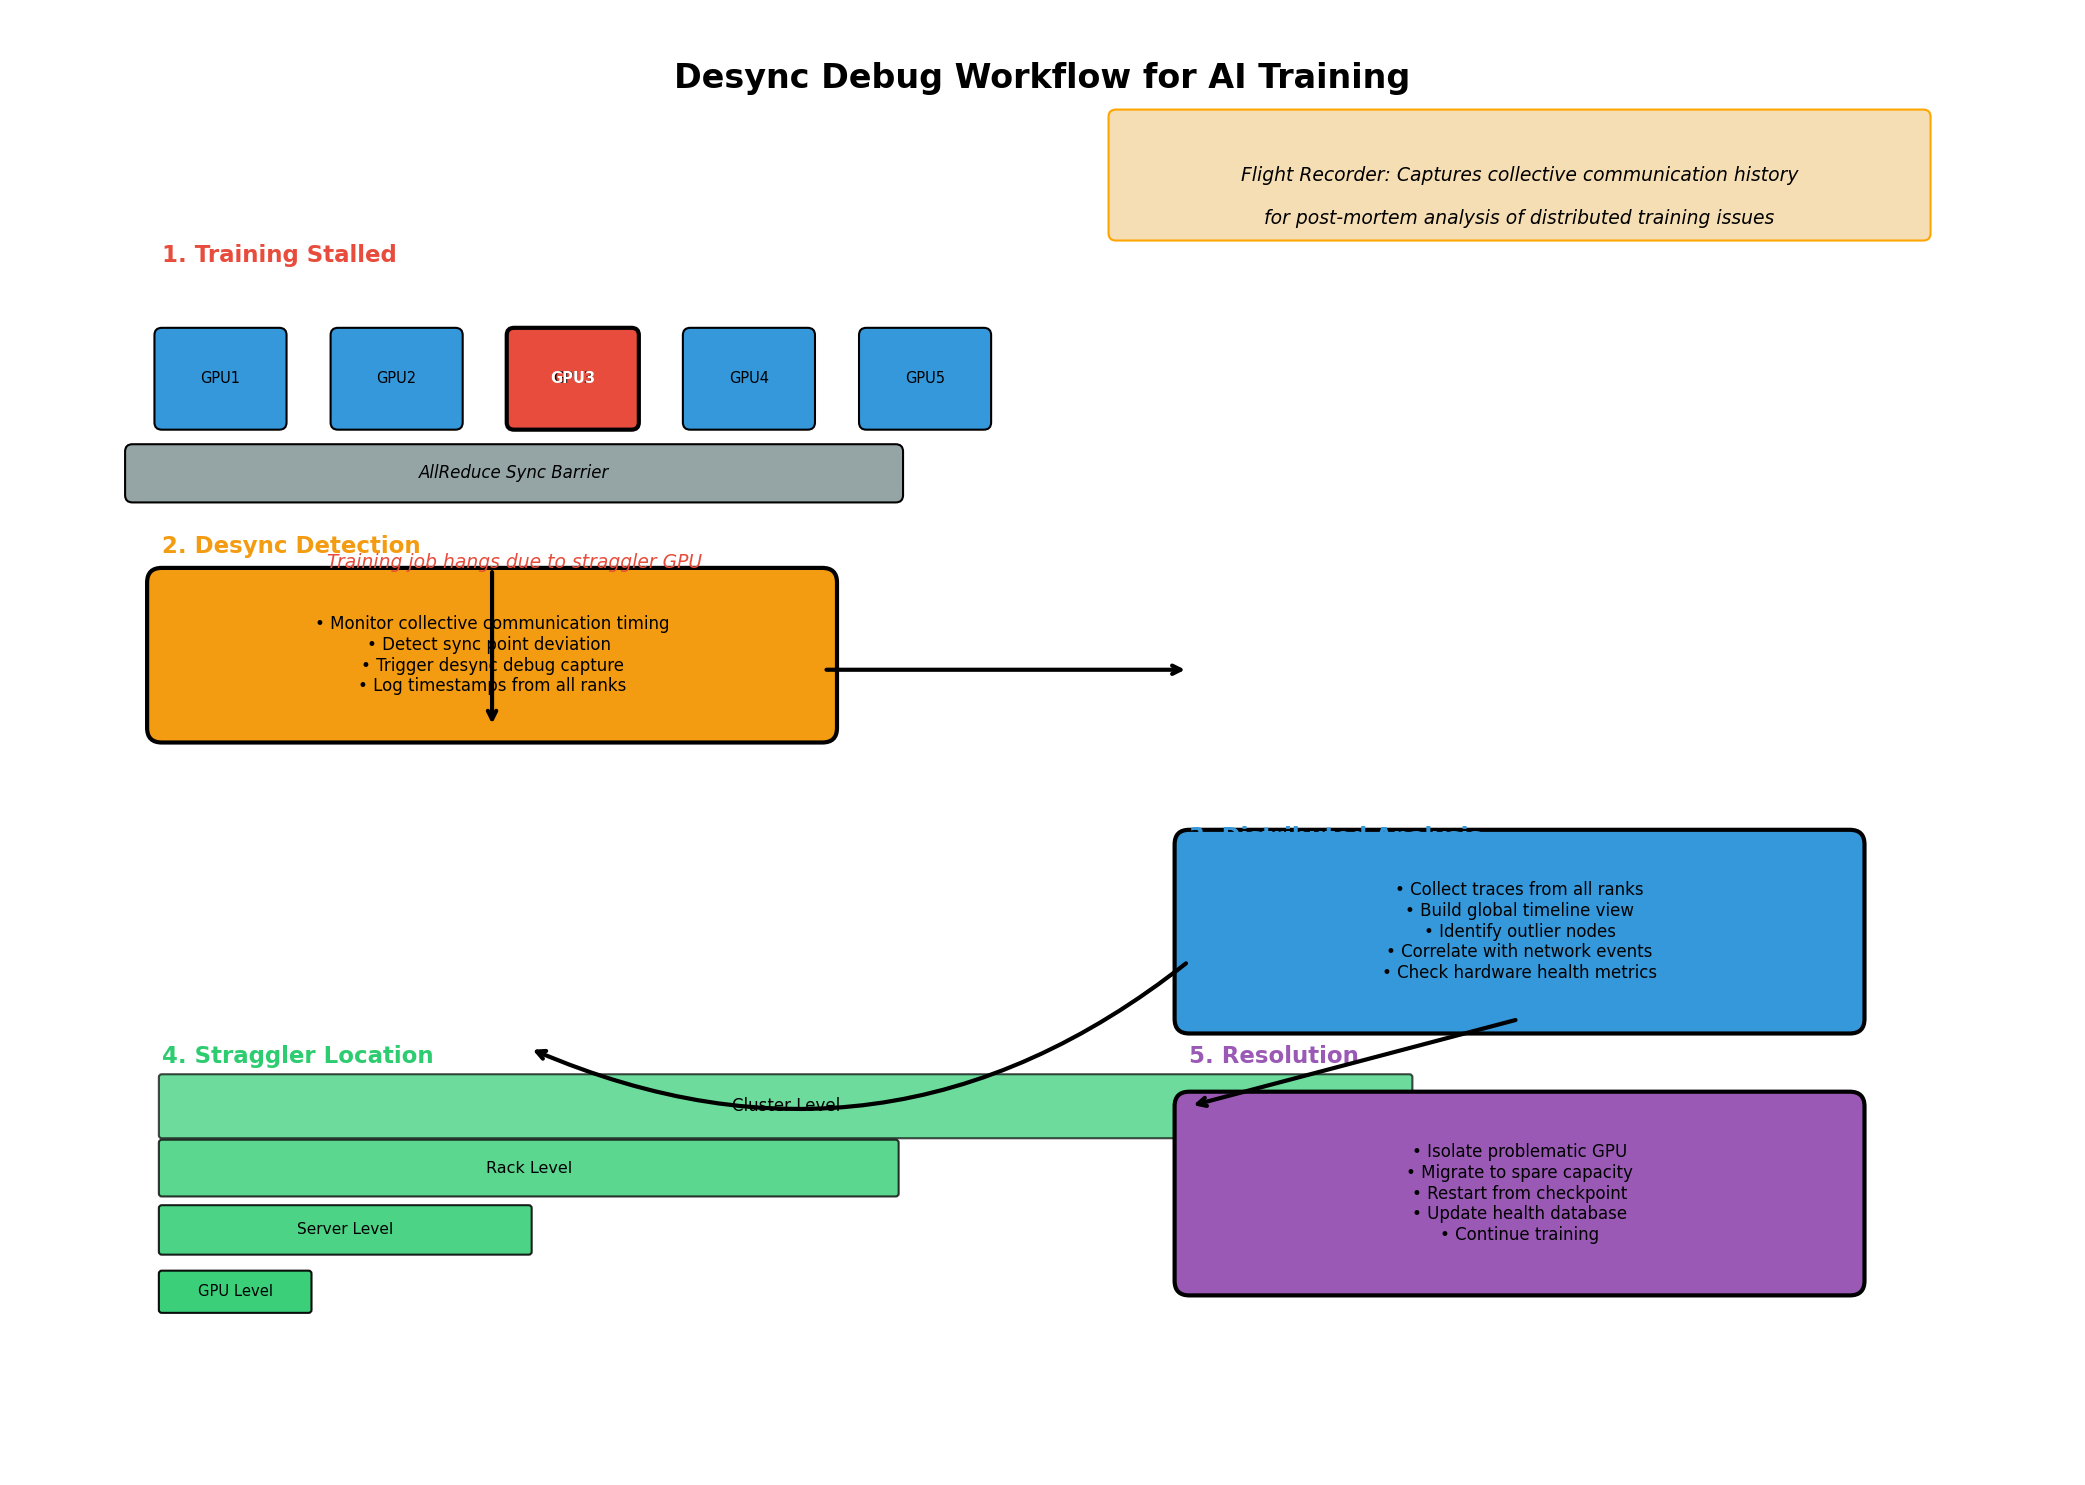
\includegraphics[width=0.95\textwidth]{assets/重构配图/ch06/fig4_desync_debug_workflow.png}
    \caption{desync debug工作流程：从检测到定位再到修复的完整流程}
    \label{fig:desync-debug}
\end{figure}

\textbf{1. desync debug工具}

desync debug的核心功能是检测集体通信中的同步延迟异常：

\begin{enumerate}
    \item \textbf{监控}：持续监控所有GPU的集体通信操作时间
    \item \textbf{检测}：识别显著偏离预期时间线的节点
    \item \textbf{关联}：将性能异常与网络事件、硬件故障关联
    \item \textbf{定位}：采用层次化方法，从集群逐步缩小到特定机架、服务器，最终定位到具体GPU
\end{enumerate}

\textbf{2. Flight Recorder（飞行记录器）}

受航空黑匣子启发，Meta开发了\textbf{分布式集合通信飞行记录器}。这个工具持续捕获集体通信的历史状态，为事后分析提供数据支持。

飞行记录器的核心价值在于：即使问题已经消失，工程师仍然可以通过历史数据还原故障场景，进行深度分析。

\subsubsection{Impact：调试效率的质变}

这些工具的应用带来了显著的运维效率提升：

\begin{itemize}
    \item 故障定位时间从数小时缩短到分钟级别
    \item 训练作业的意外中断率降低了约50倍
    \item 运维团队能够主动识别潜在问题，而非被动响应故障
\end{itemize}

更深远的影响在于，这些工具使Meta能够自信地运营更大规模的集群。随着Prometheus和Hyperion项目的推进，可调试性工具将成为基础设施的核心组成部分。

\subsection{运维万卡集群：Maintenance Trains与OpsPlanner}

\subsubsection{Problem：持续运维的挑战}

运营一个万卡GPU集群远不止硬件部署。Meta的AI基础设施团队每天需要处理：

\begin{itemize}
    \item 超过30种维护操作
    \item 50个不同组件的软件更新
    \item 三种不同的主机验证任务
    \item 数千个破坏性的AI主机任务
\end{itemize}

传统的运维方式——逐个更新、人工协调——在这种规模下完全不可行。更棘手的是，AI训练任务对中断极其敏感：

\begin{insightbox}{AI训练运维的特殊性}
\begin{enumerate}
    \item \textbf{容量保证}：许多任务无法暂停，需要24/7运行
    \item \textbf{坏主机的放大效应}：单个慢节点会影响整个集群性能
    \item \textbf{低容错率}：AI训练对中断极其敏感
    \item \textbf{一致性要求}：跨主机的软件栈必须保持一致
\end{enumerate}
\end{insightbox}

\subsubsection{Design：Maintenance Trains机制}

Meta的创新解决方案是\textbf{Maintenance Trains（维护列车）}机制。这个名字形象地描述了其工作方式：像列车一样，按固定路线、固定时间表，依次"停靠"每个维护域。

核心设计原则：

\begin{enumerate}
    \item \textbf{分域维护}：将集群划分为多个维护域，每个域独立维护
    \item \textbf{滚动更新}：一次只维护一个域，确保其他域正常运行
    \item \textbf{容量保证}：所有容量减去一个维护域24/7可用
    \item \textbf{全周期覆盖}：任何新升级都会被列车"搭载"，确保在指定时间内覆盖所有域
\end{enumerate}

维护域的大小经过精心优化。域太小会导致维护开销过大；域太大会影响容量保证。Meta与AI团队紧密合作，基于中断成本和容量损失的权衡关系，确定了最优的维护域大小。

\subsubsection{Design：OpsPlanner编排器}

Maintenance Trains解决了"何时"维护的问题，但"如何"安全地执行这些维护任务同样需要精细设计。这就是\textbf{OpsPlanner}的职责。

OpsPlanner是一个统一的工作编排器，核心能力包括：

\begin{enumerate}
    \item \textbf{范围管理}：处理重叠的操作范围，正确序列化执行
    \item \textbf{安全进出}：确保主机在维护前后正确进出生产环境
    \item \textbf{依赖管理}：确保升级按正确顺序应用（例如，先驱动后CUDA）
    \item \textbf{缓冲管理}：管理计划维护和故障缓冲区
\end{enumerate}

OpsPlanner每天处理超过100万个操作，效率极高。其内置的交接流程确保正确的升级行为，避免重叠和死锁。

\subsubsection{Safety：多层安全防护}

Meta建立了一套多层安全防护机制：

\begin{itemize}
    \item \textbf{自动停止}：如果维护或故障缓冲区耗尽，自动停止维护列车
    \item \textbf{自动回滚}：检测到升级问题时自动回滚
    \item \textbf{分阶段部署}：变更经过多阶段验证，只有经过充分测试的变更才能到达全局系统
    \item \textbf{紧急响应}：如果出现问题，可以通过紧急列车、大规模维护等方式快速响应
\end{itemize}

\subsection{小结：AI网络架构的工程智慧}

回顾Meta在AI训练网络领域的探索历程，以及公有云厂商（AWS、Google、Azure）的技术选择，我们可以提炼出几个核心工程洞察：

\begin{enumerate}
    \item \textbf{专用化胜过通用化}：当通用架构遇到根本性限制时，勇于设计专用解决方案。DSF、BAG、EFA的诞生都源于这一洞察。
    
    \item \textbf{解耦带来灵活性}：DSF通过解耦线卡和交换网板，突破了物理限制；AWS通过Nitro系统解耦网络虚拟化，实现了云原生高性能网络。
    
    \item \textbf{细粒度优于粗粒度}：包喷洒技术通过cell级负载均衡，解决了流级ECMP的根本性问题；SRD通过包喷洒实现了多租户环境下的高性能。
    
    \item \textbf{云原生vs自建各有优势}：Meta选择自建DSF追求极致控制，AWS选择EFA在公有云上提供超算能力，Google选择垂直整合TPU生态——没有绝对的优劣，只有场景适配。
    
    \item \textbf{可观测性是关键}：desync debug和Flight Recorder的开发表明，在大规模系统中，可观测性工具与基础设施本身同等重要。
    
    \item \textbf{运维即设计}：Maintenance Trains和OpsPlanner的设计表明，大规模系统的运维需要系统性的架构支持，而非临时方案。
\end{enumerate}

Meta的实践和云厂商的创新共同表明，构建下一代AI基础设施需要在网络架构、硬件选择、软件优化和运维工具等多个维度进行系统性创新。这些经验为整个行业提供了宝贵的参考。

\begin{figure}[htbp]
    \centering
    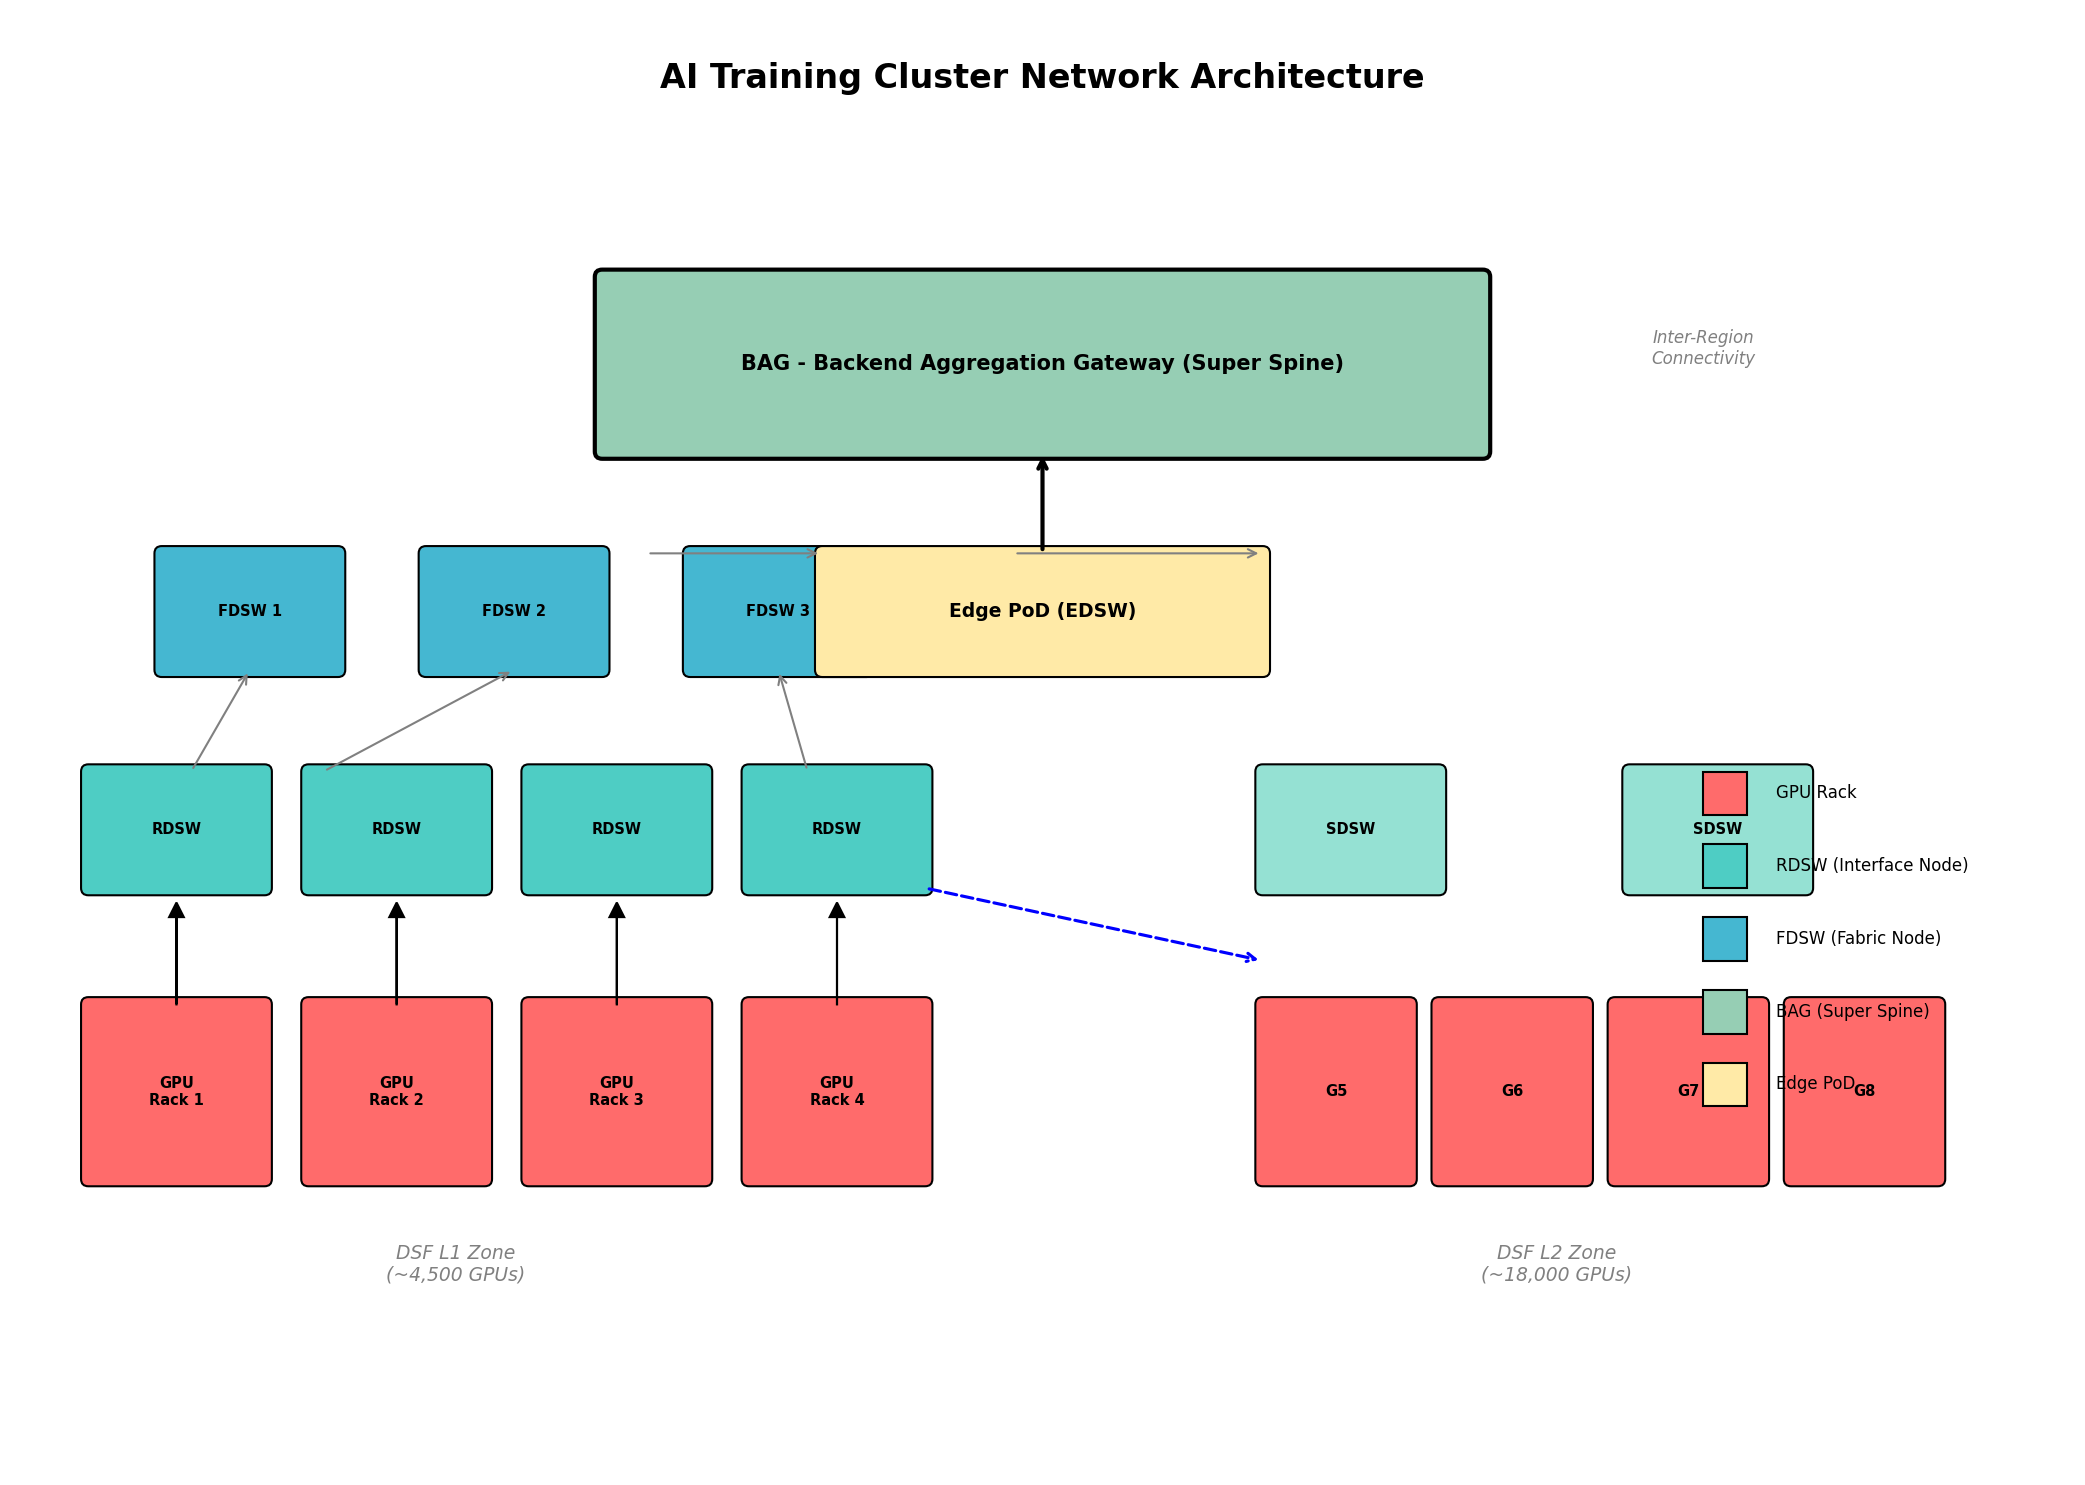
\includegraphics[width=0.95\textwidth]{assets/重构配图/ch06/fig1_ai_cluster_architecture.png}
    \caption{AI训练集群网络架构全景：从GPU机架到BAG超级脊层的完整视图}
    \label{fig:ai-cluster-architecture}
\end{figure}
% Google Ironwood TPU与AI训练网络补充
% 第6章: AI大模型训练网络
\subsection{Google Ironwood TPU：第七代AI加速器}

2025年4月，Google Cloud Next大会上，Google发布了其第七代Tensor Processing Unit (TPU)，代号Ironwood。这是Google首款专为AI推理时代设计的TPU，标志着AI基础设施从训练优先向推理优先的战略转变。

\subsubsection{Ironwood核心规格}

\begin{table}[htbp]
\centering
\caption{Ironwood TPU规格对比}
\begin{tabular}{|l|c|c|c|}
\hline
\textbf{规格} & \textbf{TPU v4} & \textbf{TPU v5p} & \textbf{Ironwood (v7)} \\
\hline
发布年份 & 2022 & 2023 & 2025 \\
单芯片峰值算力 & 275 TFLOPS & 459 TFLOPS & \textbf{4,614 TFLOPS} \\
HBM容量 & 32GB & 95GB & \textbf{192GB} \\
HBM带宽 & 1.2 TB/s & 2.8 TB/s & \textbf{7.4 TB/s} \\
芯片/Pod & 4,096 & 8,960 & \textbf{9,216} \\
Pod总算力 & - & - & \textbf{42.5 Exaflops} \\
ICI带宽 & - & - & \textbf{9.6 Tb/s} \\
制程工艺 & - & - & 3nm (TSMC N3P) \\
\hline
\end{tabular}
\end{table}

\textbf{关键性能提升：}
\begin{itemize}
    \item 相比第一代TPU（2013年）：\textbf{3,600倍}性能提升
    \item 能效提升：\textbf{29倍}
    \item 相比上一代（Trillium）：训练和推理性能提升\textbf{4倍以上}
    \item 每瓦性能：是Trillium的\textbf{2倍}
\end{itemize}

\subsubsection{Ironwood架构设计}

\textbf{1. 专为推理优化的设计}

Ironwood是Google首款专为推理时代设计的TPU：
\begin{itemize}
    \item 支持高容量、低延迟的AI推理和模型服务
    \item 针对``思考模型''（如Gemini 2.5）的计算和通信需求优化
    \item 从``响应式''AI向``主动式''洞察生成演进
\end{itemize}

\textbf{2. 芯片间互联(ICI)网络}

Ironwood采用增强的ICI网络实现大规模芯片互联：
\begin{itemize}
    \item \textbf{拓扑}：3D Torus (4x4x4) 网络结构
    \item \textbf{带宽}：9.6 Tb/s芯片间互联带宽
    \item \textbf{扩展}：最多43个64芯片块组成Superpod
    \item \textbf{共享内存}：1.77 PB共享高带宽内存
\end{itemize}

\textbf{3. 硬件配置}

\begin{itemize}
    \item \textbf{单芯片功耗}：约400W-1kW（液冷）
    \item \textbf{板级配置}：4芯片/PCBA板，16板/机架（64芯片）
    \item \textbf{Superpod规模}：144个机架，光学交换机，液冷系统
    \item \textbf{散热}：单柜可散热超过100kW
\end{itemize}

\textbf{4. AI辅助芯片设计}

Ironwood采用了Google的AlphaChip技术进行芯片设计：
\begin{itemize}
    \item 使用强化学习生成优化的芯片布局
    \item AI设计更好的AI硬件，形成正反馈循环
\end{itemize}

\subsubsection{AI Hypercomputer架构}

Ironwood是Google AI Hypercomputer架构的核心组件之一：

\begin{figure}[htbp]
\centering
\begin{tikzpicture}[scale=0.7, transform shape,
    block/.style={rectangle, draw, fill=blue!10, minimum width=3cm, minimum height=1cm, align=center},
    infra/.style={rectangle, draw, fill=green!10, minimum width=12cm, minimum height=1cm, align=center}
]
% Hardware Layer
\node[block] (tpu) at (0,0) {Ironwood TPU\\推理优化};
\node[block] (gpu) at (4,0) {NVIDIA GPU\\训练+推理};
\node[block] (cpu) at (8,0) {Axion CPU\\通用计算};

% Infrastructure Layer
\node[infra] (infra) at (6,2) {AI Hypercomputer基础设施层\\存储、网络、调度};

% Software Layer
\node[infra] (sw) at (6,4) {软件层\\Pathways, JAX, TensorFlow, PyTorch};

% Applications
\node[infra] (app) at (6,6) {应用层\\Gemini, 客户AI应用};

% Connections
\draw[->] (tpu) -- (infra);
\draw[->] (gpu) -- (infra);
\draw[->] (cpu) -- (infra);
\draw[->] (infra) -- (sw);
\draw[->] (sw) -- (app);
\end{tikzpicture}
\caption{Google AI Hypercomputer架构}
\end{figure}

\textbf{Hypercomputer关键特性：}
\begin{itemize}
    \item \textbf{灵活消费模型}：按需、预留、抢占式等多种计费方式
    \item \textbf{开放软件标准}：支持主流ML框架（JAX、TensorFlow、PyTorch）
    \item \textbf{无缝迁移}：随着新TPU代际发布，提供平滑升级路径
    \item \textbf{存储创新}：Hyperdisk Exapools、Anywhere Cache消除训练瓶颈
\end{itemize}

\subsubsection{与NVIDIA方案的竞争对比}

\begin{table}[htbp]
\centering
\caption{Google Ironwood vs NVIDIA B200对比}
\begin{tabular}{|l|c|c|}
\hline
\textbf{特性} & \textbf{Google Ironwood} & \textbf{NVIDIA B200} \\
\hline
单芯片算力 (FP8) & 4,614 TFLOPS & 4,500 TFLOPS \\
内存容量 & 192GB HBM & 192GB HBM3e \\
内存带宽 & 7.4 TB/s & 8 TB/s \\
网络 & ICI (9.6 Tb/s) & NVLink + InfiniBand \\
最大集群规模 & 9,216芯片 & 72 GPU (NVL72) \\
冷却 & 液冷 & 液冷 \\
软件生态 & Google Cloud专用 & 通用，生态更广 \\
成本模式 & 云服务订阅 & 硬件购买+云服务 \\
\hline
\end{tabular}
\end{table}

\textbf{性能估计}：分析表明Ironwood性能估计在NVIDIA B200的5\%以内，尽管采用单主计算芯片设计。

\subsubsection{TPU网络架构演进}

\textbf{Google TPU网络演进时间线：}

\begin{table}[htbp]
\centering
\caption{Google TPU代际演进}
\begin{tabular}{|l|l|l|l|}
\hline
\textbf{代际} & \textbf{年份} & \textbf{关键特性} & \textbf{应用场景} \\
\hline
TPU v1 & 2013 & 首款自研AI芯片，推理专用 & 内部搜索、翻译 \\
TPU v2 & 2017 & 支持训练，引入HBM & Cloud TPU发布 \\
TPU v3 & 2018 & 性能翻倍，液冷 & 大规模训练 \\
TPU v4 & 2022 & OCS互联，3D Torus & Pathways训练 \\
TPU v5e & 2023 & 成本优化，推理专用 & 推理服务 \\
TPU v5p & 2023 & 训练性能提升 & LLM训练 \\
Ironwood v7 & 2025 & 推理优先，42.5 Exaflops & 推理时代 \\
\hline
\end{tabular}
\end{table}

\textbf{网络拓扑演进：}
\begin{itemize}
    \item \textbf{TPU v4}：引入OCS（光电路交换）实现动态拓扑
    \item \textbf{ICI演进}：芯片间互联带宽从TPU v4的几十Gbps增长到Ironwood的9.6 Tb/s
    \item \textbf{Scale-up vs Scale-out}：Google采用收敛的主机和扩展网络设计，TPU网络既可scale-up（最多9K端点）也可scale-out
\end{itemize}

\subsubsection{对AI训练网络设计的启示}

Ironwood的发布为AI训练网络设计提供了重要参考：

\begin{enumerate}
    \item \textbf{推理优先设计}：随着AI从训练转向大规模部署，网络设计需要优先考虑推理的延迟和吞吐量要求
    
    \item \textbf{内存墙问题}：192GB HBM和7.4 TB/s带宽显示，AI芯片需要持续扩展内存容量和带宽以支持大模型
    
    \item \textbf{网络扁平化}：Google的ICI网络证明，通过高带宽、低延迟的scale-up网络可以减少对scale-out网络的依赖
    
    \item \textbf{软件协同优化}：Pathways等软件框架与硬件的深度协同是实现高效AI基础设施的关键
    
    \item \textbf{自研芯片趋势}：Google TPU的成功表明，超大规模云服务商通过自研AI芯片可以实现差异化竞争优势
\end{enumerate}

\subsection{工业实践：阿里巴巴AI训练基础设施演进}

2017年的一个深夜，阿里巴巴基础设施事业群的工程师们围坐在会议室里，面对着一块写满公式的白板。问题很简单，却令人头疼：随着集团AI业务的爆发式增长，训练一个推荐模型所需的时间已经从几小时延长到了几天，而GPU集群的利用率却始终徘徊在30\%左右。这不是硬件不够，而是整个计算架构需要重新思考。

这个场景，或许正是中国互联网巨头从"买卡堆机器"走向"系统性AI基础设施建设"的一个缩影。让我们沿着阿里巴巴的技术演进轨迹，看看一个工业级的AI训练基础设施是如何炼成的。

\subsubsection{从CPU集群到GPU集群：算法需求驱动的架构变革}

要理解阿里巴巴AI基础设施的演进，我们必须先回到那个算法与硬件相互塑造的年代。

\begin{insightbox}{机器学习发展的三个阶段}
\begin{enumerate}
    \item \textbf{1990年以前}："传统机器学习"时期，算法针对特定问题手工设计，计算需求有限，CPU足以应对。
    \item \textbf{1990-2010年}：数据驱动的统计学习时期，决策树、SVM等算法开始需要大规模数据训练，分布式CPU集群成为主流。
    \item \textbf{2010年至今}：深度学习广泛应用时期，神经网络层数从几层增长到数百层，参数规模从百万级跃升到千亿级，GPU从"图形处理器"变成了"通用并行计算引擎"。
\end{enumerate}
\end{insightbox}

阿里巴巴的机器学习实践，恰好完整经历了这三个阶段。2009年之前，集团的机器学习任务主要集中在搜索排序、广告点击率预测等场景，特征工程占主导，模型本身相对简单。那时的"大规模"训练，指的是在数百台CPU服务器上并行处理TB级的日志数据。

真正的转折点发生在2012年。当AlexNet在ImageNet竞赛中碾压传统方法的消息传来，阿里巴巴的计算机视觉团队意识到：深度学习不是学术玩具，而是即将改变整个行业的技术浪潮。但问题是——训练一个像样的深度神经网络，需要什么样的算力？

让我们做一个简单的估算。假设我们要训练一个包含10层卷积的图像分类网络，输入是224×224的彩色图像，批量大小为256。前向传播和反向传播各需要约$10^{10}$次浮点运算，一个epoch处理100万张图片，共需要100个epoch。总计算量约为：

\begin{equation}
E_{total} = 2 \times 10^{10} \times \frac{10^6}{256} \times 100 \approx 7.8 \times 10^{15} \text{ FLOPs}
\end{equation}

当时的Intel Xeon CPU峰值算力约为100 GFLOPS，单卡训练需要约22小时。而如果使用NVIDIA K20 GPU（峰值3 TFLOPS），时间可以缩短到约40分钟——这还只是一个小型网络。

当模型规模增长到数十层、参数规模达到数亿时，CPU集群已经完全无法满足需求。2014年，阿里巴巴开始大规模部署GPU集群，这是基础设施从"通用计算"向"AI专用计算"转型的起点。

\begin{figure}[htbp]
    \centering
    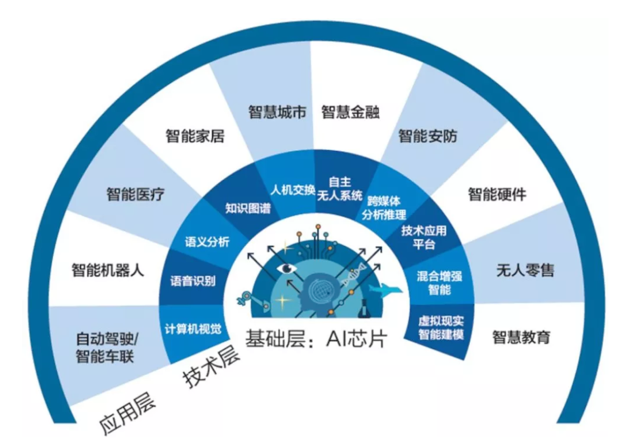
\includegraphics[width=0.9\textwidth]{assets/alibaba_20yr/alibaba20yr-13-p00-10.png}
    \caption{GPU在AI领域的应用演进：从VGA控制器到深度学习引擎的40年历程}
    \label{fig:gpu-ai-evolution}
\end{figure}

\subsubsection{内存墙问题：被数据搬运拖慢的计算}

GPU集群的部署解决了"算得慢"的问题，却暴露了一个更深层的瓶颈——\textbf{内存墙}（Memory Wall）。

让我们再次回到那个会议室。工程师们发现，即使配备了顶级GPU，训练效率仍然远低于理论峰值。监控数据显示，GPU的实际利用率经常只有20\%-40\%，大部分时间GPU都在等待数据从内存传输过来。

这就是内存墙问题的本质：\textbf{计算性能的增长速度远远快于内存带宽的增长速度}。

\begin{figure}[htbp]
    \centering
    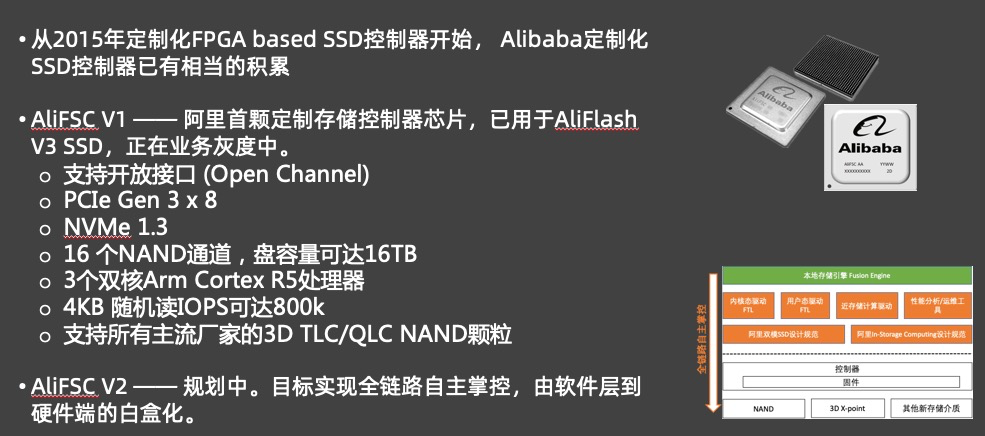
\includegraphics[width=0.85\textwidth]{assets/alibaba_20yr/alibaba20yr-13-p00-14.png}
    \caption{存储层次结构金字塔：从寄存器到磁带，容量与速度的经典权衡}
    \label{fig:memory-hierarchy}
\end{figure}

从图\ref{fig:memory-hierarchy}可以清晰地看到这个问题。处理器寄存器的访问延迟只有1个时钟周期，而主内存（DRAM）的延迟约为100个时钟周期。更糟糕的是，当数据需要从片外内存传输到计算单元时，能耗开销是惊人的——数据从内存单元传输到计算单元所需的功耗，是浮点运算本身的约200倍。

对于深度学习这种"计算相对简单、数据吞吐量巨大"的应用，内存墙的影响尤为严重。一个典型的卷积层，计算-访存比（Arithmetic Intensity）可能只有10-100 FLOPs/Byte，这意味着每读取1字节数据，只能做10-100次运算——远不足以隐藏内存延迟。

\begin{insightbox}{内存墙问题的数学本质}
设计算单元的峰值算力为$P$（FLOPS），内存带宽为$B$（Bytes/s），则计算-访存比为：
\begin{equation}
I = \frac{P}{B} \quad \text{[FLOPs/Byte]}
\end{equation}

若算法的实际计算-访存比为$I_{alg}$，则当$I_{alg} < I$时，系统受限于内存带宽（memory-bound），实际性能为：
\begin{equation}
P_{actual} = I_{alg} \times B
\end{equation}

只有当$I_{alg} \geq I$时，系统才能达到计算峰值（compute-bound）。
\end{insightbox}

既然数据搬运是瓶颈，一个直观的想法是：能不能把计算单元搬到数据旁边，甚至直接让内存"会计算"？这就是\textbf{存内计算}（Processing-in-Memory）的核心思想。

\subsubsection{存内计算：突破内存墙的架构创新}

存内计算并不是一个新概念，早在1990年代就有学者提出。但直到深度学习的广泛应用，这一技术才真正找到了"杀手级应用"。

存内计算的本质是\textbf{以内存为中心}重新设计计算架构。根据计算单元与存储单元的融合程度，可以分为三个层次。让我们用一个图书馆的类比来理解：

\begin{insightbox}{存内计算的三层架构——图书馆类比}
\begin{enumerate}
    \item \textbf{近存储计算}（Processing Near Memory）：就像在图书馆旁边建了一个计算中心。读者（数据）需要走出图书馆去计算中心处理，然后再回来。这是最容易工程化的方案，可以复用现有的IP和设计流程，但由于数据仍需在芯片间传输，性能提升有限。
    
    \item \textbf{内存储计算}（Processing In Memory）：就像在图书馆的每个阅览室里都放了一台计算器。读者不需要走出图书馆，在内部就能完成计算。这种方案可以充分利用存储芯片内部的巨大带宽（>16×），在三种技术中较好地兼顾了成熟度和性能提升。
    
    \item \textbf{内存执行计算}（Processing With Memory）：就像让书架本身会计算——你问一个问题，书架直接给你答案，连"读出来再算"的步骤都省了。这是最具革命性的方案，可以带来最大的性能和能效提升，但技术难点仍在研究中，如高效的数模/模数转换、存储单元特性分布控制等。
\end{enumerate}
\end{insightbox}

阿里巴巴在存内计算领域的布局，主要体现在两个方向：

\textbf{方向一：AI芯片的存内计算优化}

平头哥半导体在含光800等AI芯片设计中，采用了HBM（高带宽内存）技术，将内存与计算单元封装在一起，大幅缩短了数据搬运距离。HBM 2.0可以提供256 GB/s的带宽，相比传统DDR4的25.6 GB/s提升了10倍。

\begin{figure}[htbp]
    \centering
    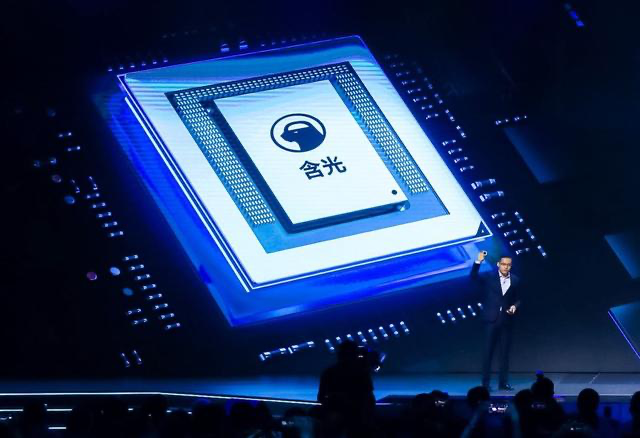
\includegraphics[width=0.8\textwidth]{assets/alibaba_20yr/alibaba20yr-13-p00-11.png}
    \caption{含光800 AI芯片：阿里巴巴首款自研神经网络加速器，专为图像视频分析和机器学习推理优化}
    \label{fig:hanguang800}
\end{figure}

\textbf{方向二：软硬件协同的访存优化}

在软件层面，阿里巴巴开发了PAI Blade编译优化工具，通过算子融合、内存复用、数据布局优化等技术，减少不必要的数据搬运。例如，将卷积、BatchNorm、ReLU三个操作融合成一个算子，可以避免中间结果写回内存，减少约30\%的内存访问量。

\subsubsection{PAI平台：大规模机器学习平台的架构演进}

如果说硬件是AI基础设施的"肌肉"，那么软件平台就是它的"神经系统"。阿里巴巴的PAI（Platform of Artificial Intelligence）平台，经历了从参数服务器（Parameter Server）到AllReduce、从单机到分布式的演进过程。

\begin{figure}[htbp]
    \centering
    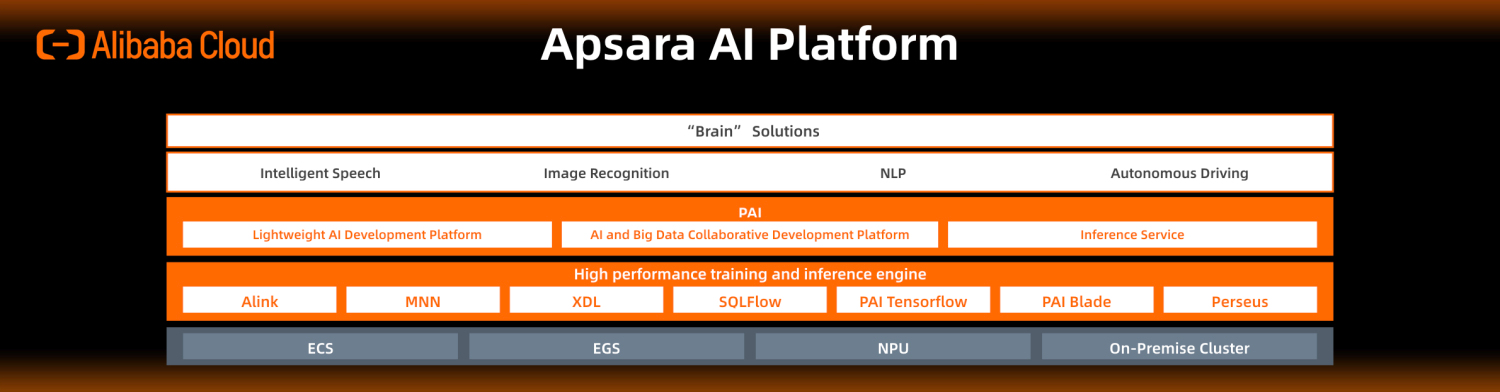
\includegraphics[width=0.95\textwidth]{assets/alibaba_20yr/alibaba20yr-11-p00-00.png}
    \caption{阿里云飞天AI平台架构：从底层ECS/EGS/NPU到上层PAI产品体系的完整技术栈}
    \label{fig:pai-architecture}
\end{figure}

\textbf{第一阶段：Parameter Server架构}

早期的分布式训练采用Parameter Server（PS）架构，这是由CMU的Eric Xing教授团队提出的一种经典范式。在PS架构中：

\begin{itemize}
    \item \textbf{Worker节点}：负责前向传播和反向传播计算，计算本地梯度
    \item \textbf{Server节点}：负责存储和更新全局模型参数
    \item \textbf{通信模式}：Worker将梯度推送给Server，Server更新参数后拉取新参数
\end{itemize}

PS架构的优势在于可以灵活处理稀疏模型（如推荐系统中的Embedding层），不同的Worker可以只更新部分参数。但PS架构也有明显的缺点：

\begin{enumerate}
    \item \textbf{通信瓶颈}：所有Worker都需要与Server通信，Server容易成为瓶颈
    \item \textbf{同步开销}：大规模集群下，同步所有Worker的进度代价高昂
    \item \textbf{扩展性限制}：当模型参数可以放入单机内存时，PS架构的效率不如AllReduce
\end{enumerate}

\textbf{第二阶段：AllReduce架构的引入}

随着深度学习模型从"宽而稀疏"（如推荐模型）向"深而稠密"（如CNN、Transformer）演进，AllReduce逐渐成为主流。

AllReduce的核心思想是\textbf{去中心化}：每个Worker都保存完整的模型副本，通过环形通信（Ring AllReduce）高效地聚合梯度。具体过程分为两个步骤：

\begin{enumerate}
    \item \textbf{Reduce-Scatter}：将梯度分块，Worker之间依次传递并累加
    \item \textbf{All-Gather}：将累加后的梯度分发给所有Worker
\end{enumerate}

对于$N$个Worker和总数据量$D$，Ring AllReduce的通信量为：
\begin{equation}
V_{comm} = 2(N-1) \times \frac{D}{N} \approx 2D \quad \text{(当$N$较大时)}
\end{equation}

这意味着即使增加更多GPU，通信总量几乎不变——就像10个人传文件和100个人传文件，总流量差不多，只是每个人传得更少了。这种特性使得系统具有良好的扩展性：增加更多GPU时，通信不会成为瓶颈。

阿里巴巴的PAI Soar分布式框架，针对深度学习同步训练场景进行了深度优化。通过融合通信、梯度压缩、混合精度等技术，在千卡规模下仍能保持85\%以上的线性加速比。

\textbf{第三阶段：超大规模稀疏模型的挑战}

推荐系统、广告点击率预测等场景，面临着独特的技术挑战——Embedding层可能包含数十亿甚至上百亿个特征，每个特征对应一个高维向量。这种\textbf{超大规模稀疏模型}的特点是：

\begin{itemize}
    \item 模型参数总量可达TB级，远超单卡显存容量
    \item 每个样本只激活极少部分参数（稀疏性>99.9\%）
    \item 需要同时处理海量样本（每天数十亿条日志）
\end{itemize}

针对这一场景，阿里巴巴开发了GRPC++分布式通信协议和EmbeddingVariable技术。EmbeddingVariable基于底层的高性能分布式KV存储，可以支持更大规模的Embedding向量，同时支持原始特征无损地直接参与模型训练。

\subsubsection{工业级训练网络的挑战与解法}

当训练集群规模从几十卡扩展到几千卡甚至上万卡时，网络通信成为决定训练效率的关键因素。阿里巴巴在这一领域的实践，为我们提供了宝贵的工程经验。

\textbf{挑战一：网络拓扑的选择}

AI训练网络需要满足几个核心需求：
\begin{enumerate}
    \item \textbf{高带宽}：AllReduce操作需要节点间持续传输大量数据
    \item \textbf{低延迟}：同步训练要求所有节点协调一致
    \item \textbf{无损传输}：RDMA通信要求网络不丢包
    \item \textbf{可扩展性}：支持从几十节点到数千节点的平滑扩展
\end{enumerate}

\textbf{InfiniBand vs RoCE的选择逻辑}

在高端AI集群中，InfiniBand（IB）和RoCE（RDMA over Converged Ethernet）是两种主流选择：

\begin{table}[htbp]
\centering
\caption{InfiniBand与RoCE技术对比}
\begin{tabular}{lcc}
\toprule
\textbf{特性} & \textbf{InfiniBand} & \textbf{RoCE} \\
\midrule
传输协议 & 原生IB协议 & 以太网+RDMA \\
延迟 & <2μs & 2-5μs \\
带宽 & 200-400 Gbps & 100-400 Gbps \\
交换机成本 & 高（专用设备） & 较低（标准以太网） \\
部署复杂度 & 需要独立网络 & 可与业务网络融合 \\
生态成熟度 & HPC领域成熟 & 云原生场景快速增长 \\
\bottomrule
\end{tabular}
\end{table}

阿里巴巴的选择是\textbf{分场景优化}：

\begin{itemize}
    \item \textbf{追求极致性能的场景}：如训练GPT-4级别的大语言模型，需要千卡甚至万卡规模的集群协同，采用InfiniBand构建独立的高性能网络。这类任务对延迟极其敏感，任何网络抖动都可能导致整个集群等待，因此值得投入专用网络的成本。
    
    \item \textbf{通用AI平台场景}：如内部推荐系统的日常迭代训练，模型规模相对较小，但需要与业务系统紧密集成，采用RoCE v2在标准以太网上提供RDMA能力。这样可以在保证性能的同时，降低部署复杂度，实现与现有网络基础设施的融合。
\end{itemize}

这种"分层解耦"的思路贯穿阿里巴巴AI基础设施的设计：不是追求单一技术的极致，而是让合适的技术解决合适的问题。

\textbf{挑战二：网络拥塞控制}

AI训练流量具有\textbf{突发性}和\textbf{同步性}特征：在AllReduce的某些阶段，所有节点会同时发送数据，形成"流量风暴"。传统的TCP拥塞控制在这种情况下表现不佳，会导致：

\begin{enumerate}
    \item 交换机缓冲区溢出，触发PFC（Priority Flow Control）风暴
    \item 队列延迟增加，RDMA性能下降
    \item 部分节点掉队，拖慢整个集群
\end{enumerate}

阿里巴巴的解决方案包括：

\begin{itemize}
    \item \textbf{ECN（Explicit Congestion Notification）}：交换机标记拥塞，发送端主动降速
    \item \textbf{PFC精细化配置}：限制PFC触发范围，避免级联效应
    \item \textbf{自适应路由}：动态选择负载较轻的路径
\end{itemize}

\textbf{挑战三：多租户资源隔离}

在公有云场景下，AI训练集群需要支持多租户共享。如何在保证性能隔离的同时，实现高资源利用率？

阿里云采用了\textbf{虚拟化RDMA}技术，通过MOC（Microcontroller on Chip）卡实现网络功能的硬件卸载：

\begin{figure}[htbp]
    \centering
    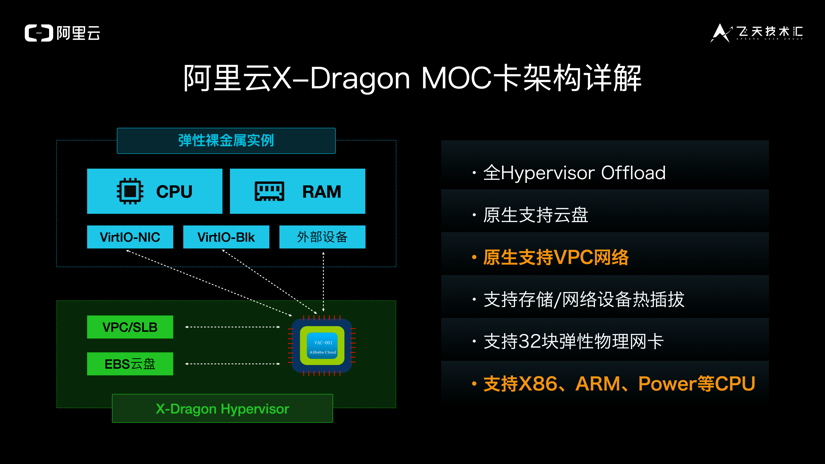
\includegraphics[width=0.9\textwidth]{assets/alibaba_20yr/alibaba20yr-13-p00-12.png}
    \caption{阿里云X-Dragon MOC卡架构：全Hypervisor卸载、原生支持VPC网络和云盘}
    \label{fig:xdragon-moc}
\end{figure}

MOC卡的核心价值在于：
\begin{enumerate}
    \item \textbf{零开销虚拟化}：网络、存储功能卸载到专用芯片，主机CPU零参与
    \item \textbf{安全隔离}：不同租户的RDMA流量在硬件层面隔离
    \item \textbf{弹性扩展}：支持热插拔，可以根据负载动态调整
\end{enumerate}

\subsubsection{演进之路的启示}

回顾阿里巴巴AI训练基础设施的演进历程，我们可以提炼出几个关键的工程洞察：

\begin{insightbox}{工业级AI基础设施的设计原则}
\begin{enumerate}
    \item \textbf{算法驱动硬件}：从CPU到GPU、从单机到分布式，每一次架构变革都源于算法需求的演进
    \item \textbf{软硬件协同优化}：存内计算、算子融合、编译优化——只有软硬一体才能突破瓶颈
    \item \textbf{分层解耦}：PAI平台通过分层抽象，让算法工程师专注于模型，让系统工程师专注于优化
    \item \textbf{场景化定制}：没有最好的架构，只有最适合特定场景的架构
\end{enumerate}
\end{insightbox}

阿里巴巴的实践表明，构建工业级AI训练基础设施是一个系统工程，需要在芯片、网络、存储、框架等多个层面进行协同创新。这些经验，与Meta的DSF/BAG、AWS的EFA/SRD、Google的TPU/OCS一起，共同构成了AI时代数据中心网络的技术图景。

% ============================================================
\section{RDMA技术：绕过内核，让GPU直接对话}
% ============================================================

\subsection{一道算术题：All-Reduce的通信账单}

我们先来做一道简单的算术题。假设你正在运行一个参数量为1750亿的GPT-3训练任务，使用了1024块A100 GPU。每完成一次迭代，每张卡需要将自己计算出的梯度与其他所有卡进行同步——这就是All-Reduce操作。

先算模型体积：1750亿个参数，以训练中常用的float16（半精度）存储，每个参数占2字节，模型总大小约为 $1750 \times 10^8 \times 2 \approx 350\text{ GB}$。在Ring-AllReduce算法中，当GPU数量 $N$ 很大时，每张卡需要发送和接收的数据量近似为 $2 \times \frac{N-1}{N} \approx 2$ 倍的模型大小，即约 $2 \times 350\text{ GB} = 700\text{ GB}$。这意味着，\textbf{每完成一次参数同步，每张GPU都需要通过网络传输约700GB的数据}。

在100Gbps的以太网链路上，仅传输时间就需要约56秒。但实际训练中，我们希望每次迭代的总时间（包括前向传播、反向传播、通信）控制在几秒以内。\textbf{通信已经成为了决定训练效率的关键瓶颈。}

更糟糕的是，传统TCP/IP网络的通信路径极其漫长。一张GPU产生梯度数据后，数据需要经历以下旅程：从GPU显存复制到CPU内存（第一次内存拷贝），CPU将数据从用户空间复制到内核的Socket缓冲区（第二次拷贝），内核协议栈进行TCP/IP封装（涉及中断处理和上下文切换），最后数据才被推送到网卡发出。接收方的过程完全对称，又是一轮逆向旅程。这一系列操作带来的不仅是延迟——\textbf{每一次上下文切换都意味着CPU被打断，而在密集训练中每秒可能发生数千次这样的中断}。整个过程就好比你要把一份文件送给隔壁同事，却必须先交给前台，前台登记、扫描、装袋，送到对方楼层的前台，再由对方前台通知同事来取。

\subsection{RDMA的核心思想：三把钥匙}

RDMA（Remote Direct Memory Access，远程直接内存访问）的诞生，正是为了打破这一僵局。它的核心思想可以用三把"钥匙"来概括。

\textbf{第一把钥匙：零拷贝（Zero-Copy）。}在RDMA模型中，数据从发送方的用户空间内存直接传输到接收方的用户空间内存，全程不经过CPU的搬运，也不经过内核缓冲区的中转。从数据的视角看，它在一次操作中完成了从源头到目的地的"直达快递"，而不是经历多次换乘的"辗转快递"。这将延迟从微秒级（$\mu$s）降低到了亚微秒级，在InfiniBand网络上典型的端到端延迟可低至1\textasciitilde2\,$\mu$s。

\textbf{第二把钥匙：内核旁路（Kernel Bypass）。}RDMA的发送和接收操作完全绕过操作系统内核，用户态程序通过RDMA网卡（RNIC）提供的专用Verbs API直接操作硬件。这意味着不再有系统调用的开销，不再有中断处理的延迟，也不再有CPU与内核之间的上下文切换。对于一个运行着数百个通信任务的AI训练集群，这一改进将CPU占用率从数十个百分点降低至接近零。\textbf{CPU从"快递员"变回了"工程师"，专注于真正的计算工作。}

\textbf{第三把钥匙：协议卸载（Protocol Offload）。}传统TCP/IP协议栈的所有处理——拥塞控制、流量控制、重传逻辑——都运行在CPU上，消耗大量计算资源。RDMA将整个传输层协议的实现迁移到了RNIC硬件芯片中。CPU只需告诉网卡"请把这块内存里的数据发送到远端的那块内存"，剩下的事情完全由网卡自主完成。这不仅解放了CPU，更重要的是为\textbf{一致、可预期的低延迟}提供了硬件级别的保证。

\subsection{三条技术路线：InfiniBand、RoCE与iWARP}

RDMA并非一种单一的协议，而是一套技术规范，目前存在三种主流的实现路线，各有其适用场景与工程权衡。

\textbf{InfiniBand（IB）}是RDMA技术的"原教旨主义"实现，从物理层到传输层完全重新设计，彻底摆脱了以太网的束缚。IB网络具有天然的无损特性，延迟极低（典型值约1\,$\mu$s），带宽极高（HDR InfiniBand可达200Gbps），是超级计算机和高性能计算（HPC）集群的首选。然而，IB网络需要专用交换机和专用网卡，与现有以太网基础设施完全不兼容，\textbf{建设成本高昂，通常是以太网方案的3\textasciitilde5倍}。英伟达的DGX SuperPOD集群、谷歌早期的TPU Pod互联均采用IB架构。

\textbf{RoCE（RDMA over Converged Ethernet）}是以太网阵营的应答：保留RDMA的语义，但将传输层运行在以太网之上。RoCEv1工作在二层，仅支持同一广播域内的通信；而\textbf{RoCEv2}将RDMA封装在UDP/IPv4或IPv6报文中，突破了二层边界，可以跨越路由器，这使得它真正具备了大规模数据中心部署的可行性。RoCE的最大优势是复用现有以太网基础设施，降低了引入RDMA的门槛。代价是：\textbf{以太网本身不保证无损传输}，必须借助PFC（Priority Flow Control，优先级流控）等机制来抑制丢包。PFC的工作原理直观：当接收端的缓冲区即将被填满时，它会向发送端发出一个"暂停信号"（PAUSE帧），要求发送端临时停止数据发送，等缓冲区腾出空间后再恢复——本质上是一种硬件级的流量控制。然而，PFC如同"双刃剑"，若控制不当，PAUSE帧可能在网络中扩散失控，引发"PFC风暴"等新的稳定性风险，后文将详述。

\textbf{iWARP（Internet Wide Area RDMA Protocol）}将RDMA运行在标准TCP之上，借助TCP的可靠传输保证，天然支持有损网络，无需PFC。iWARP的优势是兼容性极佳，\textbf{甚至可以穿越NAT和防火墙}，适合跨数据中心的广域网场景。但其局限也正在于此：TCP的连接管理和流量控制开销削弱了RDMA本应带来的性能优势，延迟通常高于RoCEv2，在密集的集群内通信中竞争力有限。

简言之：IB性能最强但成本最高，RoCEv2是主流，iWARP适合广域网。三者详细对比见表~\ref{tab:rdma_compare}。

\begin{table}[h]
\centering
\caption{三种RDMA实现技术对比}
\label{tab:rdma_compare}
\begin{tabular}{lllll}
\hline
\textbf{技术} & \textbf{典型延迟} & \textbf{最高带宽} & \textbf{无损保障} & \textbf{适用场景} \\
\hline
InfiniBand & $\sim$1\,$\mu$s & 200\,Gbps（HDR） & 原生无损 & HPC、超算、AI专用集群 \\
RoCEv2 & 1\textasciitilde3\,$\mu$s & 400\,Gbps（NDR以太网） & 依赖PFC & 数据中心AI训练、云计算 \\
iWARP & 3\textasciitilde10\,$\mu$s & 受限于TCP开销 & TCP重传保障 & 广域网、混合云、有损网络 \\
\hline
\end{tabular}
\end{table}

\subsection{阿里云的工程实践：从SCC到弹性RDMA}

理论上的三条路线在工程落地时，每一条都面临现实世界的挑战。阿里云的RDMA演进历程，是一部在规模、成本与稳定性之间寻求平衡的工程史。

\textbf{起点：神龙SCC超级计算集群。}阿里云最初为高性能计算用户推出了SCC（Super Computing Cluster）实例，基于RDMA技术提供HPC级别的网络性能。这是RDMA在阿里云的"试验田"，验证了RDMA技术在云环境中的可行性。

\textbf{转折：SMC-R与零改造的商业诉求。}然而，RDMA的编程接口（IB Verbs API）与传统Socket接口有着巨大差异，要求应用程序进行大规模改造。阿里巴巴的双十一业务中，大量成熟的分布式存储和数据库应用——如ESSD云盘、PolarDB——都基于TCP Socket编写，无法轻易切换到RDMA的Verbs API。为此，阿里云在操作系统层面实现了\textbf{SMC-R（Shared Memory Communications over RDMA）}技术：这是一套与TCP/IP并行的协议族，向上完全兼容POSIX Socket接口，向下使用RDMA完成数据传输。应用程序无需修改任何代码，只需在建立连接时协商使用SMC-R协议，就能透明地将TCP通信替换为RDMA通信。\textbf{在ESSD存储场景的大块连续I/O测试中，SMC-R使神龙实例的网络吞吐量提升约20\%}；在高并发短消息场景（如数据库访问）下，延迟降低更为显著，但绝对吞吐提升幅度因负载而异。

\textbf{突破：弹性RDMA（eRDMA）}。传统RDMA部署要求物理网卡直接暴露给虚拟机，在多租户的公有云环境中，这既带来了安全隔离的挑战，也限制了弹性扩展的能力。阿里云在第四代神龙架构中，通过基于SR-IOV的RDMA虚拟化方案实现了"弹性RDMA"（eRDMA）。SR-IOV就像把一张物理网卡"虚拟克隆"成多张独立网卡——每台虚拟机独享其中一张，性能与物理机媲美，互不干扰：具体而言，SR-IOV将物理网卡（PF，Physical Function）切分为多个虚拟功能（VF，Virtual Function），每个VM或容器独享一个VF，实现硬件级安全隔离；同时通过vSwitch硬件卸载和VXLAN隧道技术，使RDMA流量能够在VPC虚拟网络中正常转发，彻底\textbf{打破了RDMA只能在物理机或裸金属实例上使用的壁垒}。

eRDMA方案将RoCEv2封装在VXLAN隧道中传输，报文的外层是标准IPv6，内层携带完整的RoCEv2格式，ECN（Explicit Congestion Notification，显式拥塞通知——IP协议中用于向发送端告知网络拥塞状态的标志位）信息在封装和解封装时被完整保留，确保端到端的拥塞控制机制正常工作。这一方案使得普通ECS用户也能以接近物理机的性能享受RDMA带来的网络加速，将RDMA从"HPC专属的奢侈品"变成了"云上普惠的基础设施"。

\subsection{RDMA在AI训练中的实测数据}

上述技术进步最终体现为可量化的性能提升。根据阿里云内部对AI训练工作负载的测量数据，在多机多卡的分布式训练场景下：

在\textbf{AllReduce通信效率}方面，启用RoCE RDMA后，相比TCP方案，节点间梯度同步的通信时延降低60\%\textasciitilde70\%，有效带宽利用率从约40\%提升至85\%以上。以100Gbps链路为例，TCP方案由于内核协议栈开销，实际可用带宽往往仅有40\textasciitilde50Gbps；而RDMA方案能够将带宽利用率推至90Gbps以上。

在\textbf{CPU资源消耗}方面，RDMA的协议卸载效果尤为显著。在同等通信吞吐量下，RDMA方案的CPU占用率降低约80\%。这些被释放的CPU资源，可以用于数据预处理、梯度计算等真正创造价值的工作，形成良性循环。

在\textbf{端到端训练加速}方面，阿里云对Megatron-LM大模型训练的基准测试显示，从TCP切换到RDMA后，百亿参数模型的训练吞吐量（以TFLOPS/GPU衡量）提升约15\%\textasciitilde25\%，在通信-计算比较高的大模型（参数量越大，梯度体积越大）上收益更为明显。

\begin{insightbox}{为什么RDMA并非"一劳永逸"的解药}
RDMA并非没有代价。\textbf{RDMA网络对丢包极度敏感}：传统TCP有完善的选择重传机制，丢包对性能的影响是局部的、可恢复的；而RDMA的硬件重传机制相对简单——如果第N个包丢失，硬件将从第N个包开始重传之后所有的数据包，导致"一包丢失，全局等待"的灾难性后果。

为了保证零丢包，RoCEv2依赖PFC（优先级流控）机制：当接收端缓冲区快满时，向发送端发送PAUSE帧，要求其暂停发送。但PFC如同"双刃剑"——如果PAUSE帧在网络中扩散失控，可能引发\textbf{PFC风暴}，导致整个RDMA域的所有流量全部停滞；更极端的情况下，多台主机之间形成环形依赖，互相发PAUSE帧，形成\textbf{PFC死锁}，从此谁也无法发送数据。阿里云为此建立了专门的RDMA运营体系，包括快速恢复机制（检测到PFC风暴时自动关闭PFC以恢复通信）、POD庖丁丢包追踪系统，以及基于NAK的链路级丢包定位工具。

因此，RDMA更像是一辆F1赛车：极致的性能背后，需要专业的维护团队和严格的运营管控才能稳定发挥。
\end{insightbox}

从All-Reduce的通信困境出发，我们看到了RDMA如何通过零拷贝、内核旁路和协议卸载这三把钥匙，从根本上重构了数据中心的传输层；又如何在阿里云的工程实践中，从高性能计算的专用方案演化为云原生的普惠技术。然而，RDMA只解决了"传输层的效率"问题——如何保证这张高速网络在大规模集群中持续稳定运行，不出现故障，或在故障时快速定位和恢复，是下一个我们必须面对的挑战。

% ============================================================
\section{网络故障监控技术：从经验到智能的演进}
% ============================================================

\subsection{为什么网络监控如此重要}

2021年10月4日，Facebook（今Meta）发生了一次持续约6小时的全球性宕机。故障原因并非服务器崩溃，而是一次普通的网络配置变更触发了连锁反应：边界网关协议（BGP）路由被错误撤销，DNS服务随之瘫痪，进而导致全球所有服务停止响应。这次事故造成了超过640亿美元的市值蒸发，每小时直接经济损失超过40万美元。

这个例子说明了一个深刻的道理：在云计算和AI训练的时代，\textbf{网络不再是"管道"，而是整个系统的中枢神经}。任何微小的抖动都会在分布式训练集群中被放大——一台机器的网卡抖动，可能导致与它参与同一All-Reduce通信的数百台GPU全部陷入等待，整个训练任务的吞吐量骤降。

更困难的是，当业务出现性能问题时，第一个被质疑的往往是网络。阿里云基础设施团队曾对两年内500余个基础设施故障进行系统分析，发现其中不到一半真正是网络故障——服务器、电源、散热等因素同样是主要根因。网络工程师面临着一个尴尬处境：\textbf{说不清楚网络没问题，就只能背锅}。

因此，一个优秀的网络监控系统需要实现两个目标：第一，当问题不是网络造成的，能够迅速\textbf{自证清白}；第二，当真的是网络问题时，能够\textbf{快速定位}——因为阿里云的故障统计表明，在所有网络故障中，\emph{故障定位阶段耗费了整个修复过程90\%的时间}，一旦定位成功，修复往往只需几分钟。

\subsection{衡量网络稳定性的两个维度}

在讨论具体的监控技术之前，我们先要明确"稳定"意味着什么。

不妨用物流网络来类比。评价一个快递公司的好坏，最基本的标准是\textbf{能送到}——用户下单后，包裹能够到达目的地，这是可达性（Reachability）的问题。但仅仅"能送到"还不够，第二个维度是\textbf{送得快}——如果一个包裹发出后半年才到，虽然可达性没有问题，但显然不是好的物流网络。对应到计算机网络，这是\textbf{性能}（Performance）的问题，具体表现为端到端延迟是否足够低、是否存在微突发拥塞。

所谓网络监控，就是持续度量这两个指标，并在异常发生时能够迅速给出答案：\emph{网络到底有没有问题？问题出在哪里？}

\subsection{传统物理网络监控的四种方法}

面对一个数据中心——交换机将数以万计的服务器通过物理链路互联——如何监控它的稳定性？最理想的方案，是像快递追踪系统那样，记录每个数据包在每台交换机的精确时间戳和转发路径。然而，这个方案在规模上根本行不通：一个中等规模的数据中心每秒处理约\textbf{2亿个}报文，若对每个包的每跳信息都进行采集存储，所需的计算和存储资源将与被监控的数据中心本身一样庞大。

退而求其次，我们转而寻找"统计近似"的方案。历史上形成了四类典型的物理网络监控技术，它们都在阿里云、AWS、Google、Microsoft等主要云厂商的数据中心中有广泛部署。

\subsubsection{第一类：服务器主动探测（Active Probing）}

最直觉的思路：\emph{既然无法监控每个真实包，就主动发送测试包。} 就像用试探性的快递包裹来检验物流网络是否畅通。

Microsoft研发的\textbf{Pingmesh}是这类方法的代表性工作。系统在数据中心所有服务器之间建立全连接的探测网格，每台服务器定期向其他服务器发送ICMP探测报文，汇总延迟和丢包信息后，通过热力图进行可视化展示。

Pingmesh的视觉化设计尤为精妙：横轴和纵轴各排列所有服务器（按机架顺序），每个像素点代表对应服务器对之间的探测结果——绿色表示连通且延迟正常，红色表示异常。当网络完全正常时，图像应为全绿矩阵；当某个接入层交换机故障时，会出现一个方形的红色区块；若核心层交换机出问题，则图像中仅有对角线方块（同机架内服务器）为绿色，所有跨机架通信均呈红色。\textbf{故障的层级和大致位置，往往可通过图像直观判断}。

然而，主动探测存在两个根本性的局限。其一，\textbf{探测报文不能准确代表业务流量}：一方面，某些交换机故障可能对业务流量构成黑洞（因路由规则错误），但测试包恰好走了另一条路径而未受影响；另一方面，测试包可能刚好被随机丢包，而真实业务包却幸运通过，导致误报。其二，\textbf{故障定位精度有限}：探测报文从源到目的地会经过多台交换机，一旦未能到达，只能通过统计多个失败探测来猜测哪段链路出了问题，难以精确到具体的交换机或链路。

\subsubsection{第二类：应用性能统计推断（Application-Level Inference）}

如果说主动探测是"发假包看情况"，这类方法则是"观察真实业务有没有异常"——从应用层的表现反推网络是否有问题。

具体做法是在服务器上持续采集TCP重传率、RPC延迟分布、应用层吞吐量等指标，一旦某应用表现异常，就将其定性为潜在的网络故障信号。

这种方法的优势是天然基于真实流量，不存在"测试包和业务包走不同路径"的代表性问题。缺陷同样明显：应用性能受服务器负载、代码逻辑、存储系统等诸多因素影响，网络异常和应用异常混杂在一起，\textbf{相关性不等于因果性}——应用变慢了，到底是网络问题还是服务器问题，仍难以辨别。

\subsubsection{第三类：交换机统计数据上报（Switch Counter Reporting）}

这类方法让数据链路中的"中转站"——交换机，主动上报自身的统计信息：队列深度、丢包计数、错包计数、端口利用率等。就像每个快递中转站统计"到了多少包裹、损坏了多少、退回了多少"。

交换机原生支持通过SNMP（Simple Network Management Protocol）或Streaming Telemetry协议周期性地将这些计数器推送给集中式的监控系统。相比前两类方法，这类方法能够直接从硬件层面获取故障证据，是目前最成熟、部署最广泛的监控手段。

局限在于\textbf{粒度较粗，且存在信息丢失}：计数器只告诉你"端口X丢了1000个包"，却无法告诉你这1000个包属于哪条流、从哪来去往何处。此外，计数器以固定间隔（通常秒级）轮询，短暂的微突发丢包可能在下一次采集周期之前就"消化"了，完全不留痕迹。

\subsubsection{第四类：报文采样与镜像（Packet Sampling \& Mirroring）}

最后一类方法是对真实流量进行抽样检查——并不处理每个包，而是按一定比例（如1/1000）随机抽取报文进行镜像转发，发送给独立的分析器。就像海关对货物的随机抽查，检查这些"代表性样本"是否一切正常。

典型实现包括NetFlow/sFlow等协议，以及更精细的P4程序定义的报文镜像。这类方法能够保留完整的五元组（源IP、目的IP、源端口、目的端口、协议）等业务流信息，对故障根因分析提供丰富的上下文。

然而，\textbf{采样比例决定了分辨率}：采样率太低，可能错过大量异常事件；采样率太高，分析系统的处理压力又呈线性增长。此外，镜像报文本身也会占用带宽，在高速率场景下，监控系统可能成为新的瓶颈。

\subsection{四类传统方法的共同局限}

以上四类技术各有侧重，互为补充——可以将它们理解为四个不同观测角度下的"近似投影"。在实践中，阿里云、AWS等云厂商通常同时部署多种手段，通过叉乘验证来提高故障判断的置信度。

然而，无论如何组合，传统方法都面临一个\textbf{共同的天花板}：它们本质上都是间接推断，而非直接观测。

\begin{itemize}
    \item 主动探测：测试包走的路径可能和业务包不同
    \item 应用统计：应用层感知网络问题时往往已有明显延迟，且混入了非网络因素
    \item 交换机计数器：秒级轮询粒度，无法捕捉微突发；无法关联到具体流
    \item 报文采样：采样具有随机性，低概率事件很可能被遗漏
\end{itemize}

那么，有没有可能像"快递全程追踪"那样，以可控的开销实现对真实业务流量的\textbf{逐包、细粒度、全覆盖}监控？这正是阿里云网络研究团队探索的方向。

\subsection{网络可视化技术：让每个包都有"身份证"}

\subsubsection{核心思想：在数据平面直接感知异常}

阿里云AIS网络研究团队提出了一种称为\textbf{网络可视化}（Network Visibility）的技术框架，其核心思想是：\emph{不在中央控制器处间接推断，而是在每台交换机的数据平面（Data Plane）直接检测和记录报文级别的异常事件，再将这些"已经确认的事件"汇报给监控后端}。

这种范式转变的意义在于：传统方法上报的是原始数据（计数器、采样包），需要在后端进行大量关联分析才能判断有没有问题；而网络可视化方法上报的是\textbf{已经判定的异常事件}，大幅降低了后端的数据量和分析复杂度。

\subsubsection{丢包事件检测：两类不同的检测挑战}

数据中心网络中，丢包发生在两种位置，对应两种截然不同的检测机制。

\textbf{交换机内部丢包}的检测相对直接。现代可编程交换机（如Tofino系列）能够在转发流水线中对报文进行逐包编号，并在出口检查编号是否连续。一旦发现序号跳跃，即可断定有包在该交换机内被丢弃，并立即生成包含流标识符、丢包位置、时间戳等信息的异常事件。

\textbf{交换机之间链路上的丢包}（静默丢包，Silent Drop）则更为棘手。链路是光纤或电缆，本身没有可编程的"大脑"，无法自我感知。解决思路是\emph{用链路两侧的交换机夹住中间的链路}：上游交换机对报文打上序号标签，下游交换机在接收时检查序号连续性——若发现跳号，则断定链路上发生了丢包，并向监控系统上报。\textbf{比特翻转}（Bit Corruption）导致的帧错误，也可以通过这种端到端序号校验机制发现。

阿里云基础设施团队对内部网络故障类型进行了系统化分类，按故障诊断耗时由短到长大致为：交换机内部队列丢包 < 服务器网卡故障 < 交换机间链路静默丢包。\textbf{链路静默丢包虽然数量占比不高，但诊断时间极长}——因为传统方法对这种"发生在设备之间"的故障几乎无能为力——这正是网络可视化方法重点攻克的问题类型。

\subsubsection{系统工程：让高频事件可控上报}

确定了"哪里发生了什么异常"还不够，还需要解决\textbf{如何高效地将这些信息传送到监控后端}的问题。在高速网络中，丢包事件的频率可能极高，若逐一上报，监控路径本身就会成为新的瓶颈。阿里云团队设计了两个关键机制：

\textbf{事件去重}：网络故障往往"批发式"发生。一个路由黑洞可能导致某条流的所有报文都被丢弃，若对每个被丢弃的报文都生成一条事件记录，则监控后端将收到数以万计的重复信息。为此，系统在交换机内部维护一张基于哈希索引的精确匹配表，按流标识符对事件去重并累计计数器。

这里有一个微妙的工程细节：经典的Bloom Filter虽然能够实现高效的去重查找，但存在\textbf{假阴性}（False Negative）风险——当哈希表填满后，它可能误判一个新事件为"已出现过"而漏报。在网络监控场景中，漏报是不可接受的。因此阿里云的实现采用了\textbf{哈希+精确匹配表结合}的无损去重方案：通过一次哈希确定表项位置，存储精确的五元组与计数器；发生哈希冲突时，同时上报两个事件并记录计数，既避免漏报，又实现了事件聚合。

\textbf{事件批处理}：单个异常事件经过压缩后只需约24字节，但以太网最小帧长为64字节，若每个事件单独封装上报，将有约60\%的带宽用于填充冗余字节。系统通过流水线缓冲机制，将多个事件批量打包成一个MTU大小（约1500字节）的报文再上送，单帧可携带约60条事件记录，\textbf{大幅降低监控流量对生产网络的占用}。

\subsubsection{实际效果：分钟级定位，从小时缩短到秒}

阿里云在实验床上复现了历史上的5个典型P3/P4级网络故障——这些故障由于定位时间漫长，最终均升级为S2级严重事故——并使用网络可视化技术重新进行诊断。结果表明，\textbf{这些复现故障均可在1分钟以内完成精确定位}，相比传统手段下数小时乃至数天的排查周期，效率提升超过两个数量级。

直觉上这不难理解：当一台服务器的业务报文在某台交换机上被丢弃时，网络可视化方法能直接告诉你"是哪台交换机，哪个端口，丢了多少个属于哪条流的包"——这正是传统监控手段最难给出的答案。

\subsection{未来展望：从监控到自愈}

网络可视化技术解决了"看得见"的问题，但这只是第一步。当网络能够实时感知自身的每一处异常时，自然会引出下一个问题：\emph{除了告警，能不能直接处理？}

\textbf{方向一：网络内自动绕路（In-Network Fast Reroute）}

传统的故障恢复流程是：监控系统检测到异常 → 上报告警 → 网络工程师介入分析 → 下发修复命令。这个流程即便顺利，也需要分钟级的响应时间。在AI大模型训练场景中，分钟级的网络中断意味着数百个GPU的训练中断——这是不可接受的。

更理想的模式是：交换机在检测到某条路径丢包后，\textbf{在硬件流水线内直接将受影响的流量切换到备用路径}，整个绕路过程发生在微秒量级，应用层无感知。故障的"慢修"（替换硬件）可以异步进行，而业务始终保持正常运转。这种"先绕后修"的思路，将网络的可靠性从"快速恢复"推向了"无损运行"。

\textbf{方向二：通用可编程测量框架（Sketch-based Network Measurement）}

随着网络研究的深入，运营团队对网络数据的需求愈发多样化：哪些流量是"超级发送者"（Superspreader）？队列突发（Burst）在一天中的分布规律是什么？不同服务类型的流量比例如何变化？

为了满足这些\textbf{定制化测量}的需求而不必每次重新设计硬件，学术界正在探索基于\textbf{Sketch}的可编程测量框架。Sketch脱胎于流式处理领域，能够用有限的内存和计算资源实现对数据流的多种统计摘要——计数、频率估计、分位数统计等。将Sketch引入可编程交换机的流水线，可以构建一个\textbf{用数据平面程序就能灵活定义测量逻辑}的通用框架，无需修改硬件即可适配新的测量需求。

\subsection{本节小结：监控能力决定运营边界}

回顾本节介绍的网络监控技术演进，有一条主线始终清晰：\textbf{可观测性（Observability）决定了运营能力的上限}。

从四类传统方法（主动探测、应用推断、计数器上报、报文采样）的间接近似，到网络可视化技术对真实业务流量的逐流事件感知，再到未来网络内自愈和通用测量框架，每一次进步的本质都是\textbf{让网络对自身状态的认知更加精准、及时、可操作}。

对于本书关注的AI大模型训练网络而言，这一趋势尤为重要：当训练集群规模达到数万GPU、通信模式高度周期性时，任何一处持续的静默丢包都会在全局性能指标中留下清晰的指纹。\textbf{网络可视化提供的精细感知能力，是运营大规模训练集群的必要前提，而非锦上添花的高级功能}。

\section{网络可视化系统：让流量"看得见、摸得着"}

上一节我们讨论了网络故障监控技术的演进，从传统的四类方法（主动探测、应用推断、计数器上报、报文采样）到基于网络可视化的事件感知。这一节我们将更深入地探讨网络可视化系统的完整架构与工程实践——这是阿里云从2017年开始探索、历经三年才逐步成熟的技术体系。

如果说传统监控是"看X光片"——通过间接指标推测网络内部状态，那么网络可视化就是"做内窥镜"——直接观察每一个数据包在网络设备中的真实经历。这种从"间接推断"到"直接观测"的范式转变，彻底改变了数据中心网络的运维方式。

\subsection{从无人区到引领业界：可视化的起点}

2017年，阿里云网络团队面临一个尴尬的现实：每当业务方反馈"应用超时"、"访问变慢"时，网络团队往往是最先被怀疑的对象。这种"背锅"困境源于一个根本性的信息不对称——网络服务提供者看到的是交换机、光纤、路由协议，而网络使用者（应用开发者）看到的只是延迟、超时、重传。

让我们用一个物流的类比来理解这个困境。物流公司关注的是中转站选址、路径规划、吞吐能力提升；但寄件人只想知道：我的包裹到哪了？有没有丢？什么时候能到？在网络世界里，这个"包裹"就是数据包，而长期以来，网络对应用来说完全是一个黑盒。

\textbf{网络可视化的本质目标}，就是要像物流追踪系统一样，让每一个数据包的状态对应用可见：它经过了哪些设备？在每个设备中停留了多久？是否发生了丢包？丢包原因是什么？

阿里云从2017年开始在网络可视化领域进行深度探索。这是一个真正的"技术无人区"——业界没有成熟的解决方案，学术界也仅有少量理论研究。当时团队面临三大挑战：

\textbf{挑战一：芯片能力限制}。2017年的商用交换机芯片对INT（In-network Telemetry）的支持非常有限，大部分芯片只能做简单的报文镜像，无法插入自定义元数据。团队不得不与芯片厂商深度合作，甚至参与下一代芯片的功能定义。

\textbf{挑战二：数据处理能力不足}。INT数据量巨大，传统的日志处理系统（如ELK）完全无法应对。团队需要从零构建一套能够处理每秒数亿条记录的高性能数据流水线，这涉及DPDK、P4可编程交换机、流式计算等多个前沿技术的整合。

\textbf{挑战三：业务价值证明}。作为一个"研究性质"的项目，可视化在初期很难证明其业务价值。团队需要在不影响生产稳定的前提下，逐步验证技术的可行性，这需要极大的耐心和坚持。

项目初期经历了各种质疑——"为什么要花这么大精力做可视化？SNMP不够用吗？"、"INT数据量这么大，会不会影响业务性能？"、"这个技术真的能定位问题吗？"更糟糕的是，项目核心成员在关键时刻离职，让本就艰难的项目雪上加霜。但团队始终坚信这个方向的价值，得到了领导层的支持后，继续推进。

转机出现在2018年的一次重大故障。某核心存储集群出现间歇性性能下降，业务方怀疑是网络问题，但网络团队通过传统手段完全找不到异常。可视化团队紧急部署了INT探针，仅用10分钟就定位到问题根源——某台交换机的特定队列存在周期性拥塞，原因是该队列与其他高优先级流量共享缓冲区。这是可视化技术第一次在生产环境中"证明了自己"。

经过三年的坚守，阿里云不仅连续两年在ACM SIGCOMM上发表网络可视化相关论文（SIGCOMM'19《HPCC: High Precision Congestion Control》、SIGCOMM'20《Flow Event Telemetry on Programmable Data Plane》），更在生产环境中实现了规模化部署。到2020年，可视化系统已经覆盖阿里云数十个数据中心，成为网络运维的"标配"工具。

\subsection{可视化监控系统的整体架构}

网络可视化系统的核心是基于可视化数据建立的数据收集、存储、分析系统，作为底座为监控系统和工具提供更细粒度的监控和故障定位能力。让我们从数据流动的视角来理解这个系统的整体架构。

\subsubsection{数据源：交换机和服务器}

在数据中心网络中，交换机和业务服务器作为可视化系统的数据源头，主要提供两类数据：INT（In-network Telemetry）和MOR（Mirror on Retransmission）。

\textbf{INT数据}：在5.1/5.2网络架构中，交换机芯片提供了对特定报文（如特定DSCP值）进行复制并根据特定格式插入交换机信息的能力。INT报文中包含的信息包括：进出端口时间戳、交换机设备ID、端口和队列ID等。通过INT报文，系统可以获取某条流量所经过的交换机设备路径、延时、拥塞等信息。

\textbf{MOR数据}：根据业务流量特征，交换机可以匹配特定流量并通过ERSPAN镜像到可视化后端系统。一个典型的应用是对重传报文进行镜像，即Mirror on Retransmission。系统通过分析MOR报文，可以对持续丢包进行监控告警，结合INT数据提供的路径信息定位丢包位置。

\subsubsection{后端收集系统：NetSeer Collector}

可视化后端收集系统由分布式部署的x86 DPDK服务器和P4可编程交换机构成。利用DPDK或P4可编程交换机的高性能包处理能力，后端收集系统对可视化数据进行初步的去重、过滤、汇聚处理，并将整理后的结构化数据上报至存储中间件SLS（阿里云日志服务）。

这里有一个关键的工程细节：在高速网络中，丢包事件的频率可能极高，若逐一上报，监控路径本身就会成为新的瓶颈。系统设计了两种关键机制来解决这个问题：

\textbf{事件去重}：网络故障往往"批发式"发生。一个路由黑洞可能导致某条流的所有报文都被丢弃。系统在交换机内部维护一张基于哈希索引的精确匹配表，按流标识符对事件去重并累计计数器。值得注意的是，经典的Bloom Filter虽然高效但存在假阴性（False Negative）风险——当哈希表填满后可能误判新事件为"已出现过"而漏报。在网络监控场景中，漏报是不可接受的。因此阿里云采用了\textbf{哈希+精确匹配表结合}的无损去重方案。

\textbf{事件批处理}：单个异常事件经过压缩后只需约24字节，但以太网最小帧长为64字节。系统通过流水线缓冲机制，将多个事件批量打包成一个MTU大小（约1500字节）的报文再上送，单帧可携带约60条事件记录，大幅降低监控流量对生产网络的占用。

\subsubsection{数据处理与消费}

可视化后端系统将数据上报至SLS后，依据不同的业务场景，利用Blink（阿里云流计算引擎）对数据做进一步处理，最后持久化至OTS、Hologres等存储中间件。

可视化系统通过两种方式对外提供数据消费服务：
\begin{enumerate}
    \item \textbf{实时监控告警}：利用Blink直接对SLS中的数据进行处理，对接北斗系统的"庖丁"和"无人值守"模块，提供实时告警能力。
    \item \textbf{通用数据服务}：通过可视化控制器（NetSeer Controller）对外提供API，支持上层应用按需查询网络状态。
\end{enumerate}

\subsection{下一代Telemetry：基于自研交换机的实时感知}

网络可视化的核心能力依赖于交换机对数据包的精确标记能力。让我们再次回到物流的类比：当我们查看淘宝订单的物流信息时，能看到包裹何时到达集散中心、何时装车发出——这些信息来自每个中转站对包裹的扫描记录。网络可视化要实现的正是类似的"扫描"能力。

\subsubsection{INT技术的三个关键要素}

实现网络可视化需要三个关键要素。让我们通过一个具体的例子来理解INT的工作流程：假设主机A向主机B发送一个数据包，这个包需要经过3台交换机（ToR→Leaf→Spine）。在没有INT的情况下，我们只能知道"A发了包，B收到了包"，中间发生了什么完全不可见。有了INT之后，每一台交换机都会在数据包经过时"打卡"，记录关键信息。

\textbf{要素一：精准的包标记}。交换机需要对经过的数据包进行精准标记，记录数据包进入和离开交换机的时间戳、经过的端口和队列等信息。具体来说，当INT-enabled的数据包到达交换机时，交换机会在包的特定位置（通常是尾部）插入一段元数据，包括：
\begin{itemize}
    \item \textbf{设备ID}：8字节，标识这台交换机的唯一编号
    \item \textbf{入端口ID}：2字节，数据包从哪个端口进入
    \item \textbf{出端口ID}：2字节，数据包从哪个端口离开
    \item \textbf{入时间戳}：8字节，纳秒级精度，记录进入时间
    \item \textbf{出时间戳}：8字节，纳秒级精度，记录离开时间
    \item \textbf{队列深度}：4字节，记录数据包在出端口队列中的位置
    \item \textbf{队列拥塞标记}：1字节，是否遇到ECN标记
\end{itemize}

一个数据包经过3台交换机后，会携带约100字节的INT元数据。这些元数据在数据包到达接收端主机后，由网卡提取并通过专用通道（如ERSPAN）发送到可视化后端系统。

\textbf{要素二：高性能的后端处理}。INT报文的数量可能是业务流量的数倍（取决于采样率），后端收集系统需要具备线速处理能力。以一个100Gbps的端口为例，如果INT采样率为1\%（即每100个包采样1个），那么每秒产生的INT报文数量约为：
\[
\frac{100 \times 10^9 \text{ bps}}{8 \times 1500 \text{ bytes}} \times 1\% \approx 83,000 \text{ 包/秒}
\]
这还只是单个端口。在拥有数千台交换机的数据中心中，INT数据总量可达每秒数亿条。阿里云采用DPDK和P4可编程交换机相结合的方式：DPDK服务器负责高密度的INT报文接收和初步解析，P4可编程交换机负责流级别的聚合和过滤，确保在高流量场景下不丢包、不延迟。

\textbf{要素三：智能的数据分析}。原始的可视化数据是海量的，需要通过流式计算进行实时分析，提取有价值的网络事件。分析引擎需要完成以下计算：
\begin{enumerate}
    \item \textbf{路径重构}：将同一流的多个INT记录按时间顺序拼接，还原完整转发路径
    \item \textbf{逐跳延时计算}：$\text{Delay}_i = \text{TS}_{\text{out},i} - \text{TS}_{\text{in},i}$，计算每跳交换机的处理延时
    \item \textbf{拥塞检测}：当队列深度超过阈值或出现ECN标记时，判定该跳存在拥塞
    \item \textbf{异常聚合}：将同一时间段、同一设备的异常事件聚合成有意义的告警
\end{enumerate}

\subsubsection{自研交换机的优势}

相比商用交换机，自研交换机在可视化能力上有显著优势：

\begin{itemize}
    \item \textbf{灵活的标记策略}：可以根据业务需求自定义INT标记的触发条件和内容格式
    \item \textbf{高精度时间戳}：支持纳秒级的时间戳精度，满足延时敏感业务的测量需求
    \item \textbf{可编程流水线}：支持P4语言编程，可以灵活定义数据包处理逻辑
    \item \textbf{高稳定性上报}：针对Telemetry场景优化的硬件设计，确保监控数据不丢失
\end{itemize}

阿里云在实验床上复现了历史上的5个典型P3/P4级网络故障——这些故障由于定位时间漫长，最终均升级为S2级严重事故——并使用网络可视化技术重新进行诊断。结果表明，\textbf{这些复现故障均可在1分钟以内完成精确定位}，相比传统手段下数小时乃至数天的排查周期，效率提升超过两个数量级。

\subsection{RDMA网络的可视化挑战}

RDMA（Remote Direct Memory Access）网络为可视化带来了特殊的挑战。RDMA通过内核旁路和协议卸载实现了微秒级延时，但这也意味着传统的基于内核的监控手段完全失效。更关键的是，RDMA网络通常运行在"无损"模式下，依赖PFC（Priority Flow Control）进行流量控制——一旦PFC机制出现问题，可能引发灾难性的PFC风暴。

\subsubsection{RDMA可视化的核心难点}

\textbf{难点一：静默丢包检测}。RDMA网络中的丢包往往不会触发TCP的重传机制（因为RDMA使用自己的可靠传输机制），传统的基于TCP重传的监控方法无法发现RDMA的丢包问题。在RDMA的可靠连接（RC）模式下，丢包由网卡硬件自动重传，应用层完全无感知。这意味着即使网络中存在持续丢包，应用层看到的只是延时增加，而不知道发生了丢包。更糟糕的是，如果丢包率很低（如0.001\%），对单个连接的影响微乎其微，但当数千个GPU同时训练时，这种"静默丢包"会累积成显著的性能下降——训练吞吐量可能下降10\%甚至更多，而运维人员却找不到原因。

\textbf{难点二：PFC风暴定位}。PFC风暴是RDMA网络最大的风险之一。要理解PFC风暴，首先需要理解PFC（Priority Flow Control）的工作原理。PFC是一种基于优先级的流量控制机制，当某个端口的接收缓冲区即将溢出时，交换机会向上游发送一个PFC暂停帧（Pause Frame），要求上游在指定时间内停止发送该优先级的流量。上游收到暂停帧后，会立即停止发送，直到收到恢复帧或超时。

PFC风暴的产生机制可以用一个"多米诺骨牌"的连锁反应来解释：
\begin{enumerate}
    \item \textbf{初始拥塞}：某台服务器的网卡处理速度变慢（可能是CPU负载高或应用阻塞），导致其连接的交换机端口接收缓冲区堆积
    \item \textbf{一级反压}：交换机向该端口的上游（Leaf交换机）发送PFC暂停帧
    \item \textbf{二级反压}：Leaf交换机的对应端口被暂停后，其缓冲区也开始堆积，进而向其上游（Spine交换机）发送PFC暂停帧
    \item \textbf{三级扩散}：Spine交换机被暂停后，会影响所有连接到它的Leaf交换机，即使这些Leaf交换机下的其他端口并没有拥塞
    \item \textbf{全网瘫痪}：在极端情况下，PFC暂停信号可能在整个网络中传播，导致所有RDMA流量被冻结，形成"死锁"
\end{enumerate}

一次典型的PFC风暴可能在毫秒级时间内扩散到整个POD（Pod of Data center），导致数百台服务器的RDMA通信中断数秒。由于PFC是硬件机制，一旦触发，软件层面几乎无法干预。因此，\textbf{预防}和\textbf{早期发现}是应对PFC风暴的唯一手段。

可视化系统通过实时监控每个端口的PFC帧发送/接收计数器，可以绘制出PFC传播的"热力图"。当发现某个端口的PFC发送速率异常升高时，立即触发告警并自动定位到源头设备。更进一步，结合INT数据，可以分析出触发PFC的具体流量特征（如哪个源IP、哪个DSCP值、多大的突发流量），为后续的流量工程优化提供数据支撑。

\textbf{难点三：微突发（Microburst）观测}。RDMA流量往往呈现高度突发性，微秒级的突发流量可能导致交换机队列瞬间拥塞。传统的分钟级监控完全无法捕捉这类事件。

微突发的产生与RDMA的通信模式密切相关。在大规模AI训练中，All-Reduce操作会导致数千个GPU同时发送数据，形成一个同步的"流量洪峰"。虽然每个GPU的发送速率可能只有10Gbps，但汇聚到交换机端口的瞬时流量可能达到数百Gbps，远超端口带宽（如100Gbps）。这种突发通常只持续几十到几百微秒，但足以导致交换机队列瞬间填满，触发ECN标记甚至丢包。

传统的SNMP监控以分钟为粒度，看到的只是平均流量，完全无法发现微突发。可视化系统通过INT提供的队列深度信息，可以精确到微秒级地观测每个端口的队列变化。当发现队列深度在短时间内（如10微秒）从0增长到接近最大值时，即可判定发生了微突发。通过分析微突发的发生规律（如是否与特定的All-Reduce模式相关），可以指导网络参数调优（如调整ECN阈值、增加队列深度等）。

\subsubsection{阿里云RDMA可视化方案}

针对上述挑战，阿里云设计了专门的RDMA可视化方案：

\textbf{方案一：基于INT的逐包追踪}。通过INT技术，记录每个RDMA数据包在网络中的完整路径和延时，精确识别拥塞点。

\textbf{方案二：PFC事件实时监控}。在交换机层面实时统计PFC帧的发送和接收情况，建立PFC风暴预警机制。当检测到异常数量的PFC帧时，立即触发告警并自动定位源头。

\textbf{方案三：队列深度可视化}。利用交换机提供的队列深度计数器，实时监控每个端口的队列状态，发现微突发事件的规律。

\subsection{Solar可视化：AI训练集群的专属监控}

Solar是阿里云自研的高性能通信协议，为存储和计算分离架构提供数据中心级别的稳定、高效、高性能、大规模高速网络互连能力。Solar-Leap协议深度集成了网络可视化能力，实现了细粒度的监控和故障定位。

\subsubsection{Solar可视化系统架构}

Solar可视化系统的数据链路包括：

\textbf{数据源层}：交换机和Solar服务器提供INT和MOR数据。INT用于获取流量路径和延时信息，MOR用于检测重传事件。

\textbf{收集层}：NetSeer Collector负责数据收集和初步处理，包括去重、过滤、汇聚等操作。

\textbf{处理层}：数据上报至SLS后，通过Blink进行流式处理，提取关键网络事件。

\textbf{消费层}：监控系统（如庖丁、无人值守）消费处理后的数据，提供告警和可视化展示。

\subsubsection{Solar可视化的典型应用场景}

\textbf{场景一：块存储SLA保障}。通过可视化数据，实时监控存储流量的延时分布，发现影响SLA的异常流量。

\textbf{场景二：流控异常定位}。当Solar检测到重传事件时，结合INT数据快速定位是网络拥塞还是接收端处理慢导致的。

\textbf{场景三：端口故障诊断}。当某个端口出现丢包时，可视化数据可以精确显示受影响的流量范围和业务影响。

\textbf{场景四：交换机配置错误检测}。通过对比预期路径和实际路径，发现因配置错误导致的流量绕行或黑洞。

\subsection{双十一大考：万亿流量下的实时可视化}

双十一全球购物狂欢节是阿里云网络每年面临的最大考验。2020年双十一前，阿里云在部分网络集群（EU126-VM-G5、NA62-VM-G4、NA61-VM-G2、NA62-APPDB-G5）的超过7万台服务器上部署了支持可视化的PingMesh新版本。

\subsubsection{PingMesh可视化的价值}

PingMesh是阿里自研的专门用于网络设备监控的产品，通过在不同主机之间周期性地全量互ping，收集全网ASW（接入交换机）、PSW（汇聚交换机）、DSW（核心交换机）内部与之间主机网络质量数据。但传统PingMesh存在两个不足：

\textbf{不足一}：无法得知探测流量的精确路径，无法做到全链路覆盖。如果故障链路刚好没有PingMesh流量经过，则不会有任何感知。

\textbf{不足二}：虽然可以知道端到端延时，但无法获取每一跳的延时。当延时激增时，无法判断是在哪一跳发生了拥塞。

可视化技术恰好弥补了这些不足。融合可视化能力后，PingMesh可以提供：
\begin{itemize}
    \item 网络端到端逐跳延时及端到端延时
    \item 网络流量的精确路径信息
    \item 网络各个路径的流量负载情况
    \item 网络各个路径的连通性及盲点区域信息
\end{itemize}

\subsubsection{双十一数据分析成果}

在2020年10月31日至11月12日期间，可视化系统采集了超过\textbf{980亿条}可视化数据，覆盖应用分组1100余个，DSW 96台，PSW 1136台，ASW 5301台。

数据分析揭示了几个关键发现：

\textbf{发现一：热点应用识别}。通过可视化数据可以从延时角度揭示网络压力，进而反映相关业务的负载水位。例如，在NA61-VM-G2网络集群中，AY300J应用分组在双十一零点前后的延时出现明显上涨，这与业务方的监控数据相互印证。

\textbf{发现二：RDMA业务负载可视化}。对于部署RDMA的应用分组（如AY258U），可视化数据可以精确展示其网络延时变化趋势。双十一零点过后，该分组的网络延时显著上涨，在零点到一点之间达到高峰，然后逐步走低——这与RDMA流量监控数据高度一致。

\textbf{发现三：盲点区域发现}。通过分析流量路径覆盖情况，可以发现网络中的"盲点"——那些没有被任何监控流量覆盖的链路和设备。

\subsection{NetSeer：从监控走向智能诊断}

网络可视化解决了"看得见"的问题，但运维人员真正需要的是"看得懂"。面对海量的可视化数据，如何快速定位问题根因？这是NetSeer系统要解决的核心问题。

\subsubsection{NetSeer的研究成果}

NetSeer是阿里云网络可视化项目的研究成果，其核心理念是将可视化数据与智能诊断算法相结合，实现从"被动监控"到"主动诊断"的转变。

NetSeer的主要能力包括：

\textbf{能力一：路径异常检测}。通过对比历史路径数据和实时路径数据，自动发现路由变化、流量绕行等异常。具体算法流程如下：
\begin{enumerate}
    \item \textbf{路径特征提取}：对于每一条流，提取其INT路径特征，表示为一个有序序列 $P = (S_1, S_2, ..., S_n)$，其中 $S_i$ 表示第 $i$ 跳的交换机ID和出端口
    \item \textbf{基线建立}：在正常情况下，同一类型的流（如同一应用分组内的流）通常具有相似的路径。NetSeer通过聚类算法建立每类流的"期望路径"基线
    \item \textbf{异常检测}：实时路径 $P_{\text{real}}$ 与期望路径 $P_{\text{base}}$ 对比，计算差异度 $D = \text{EditDistance}(P_{\text{real}}, P_{\text{base}})$。当 $D > \theta$（阈值，通常取2）时，判定为路径异常
    \item \textbf{根因定位}：如果多条流同时出现相同的路径变化（如都多了一跳 $S_x$），则判定 $S_x$ 可能是新加入的中间设备或发生了路由收敛
\end{enumerate}

\textbf{能力二：延时异常定位}。基于INT数据提供的逐跳延时信息，精确识别延时异常发生的具体设备和端口。算法流程如下：
\begin{enumerate}
    \item \textbf{逐跳延时分解}：对于端到端延时 $T_{\text{total}}$，分解为各跳延时之和 $T_{\text{total}} = \sum_{i=1}^{n} T_i$，其中 $T_i = \text{TS}_{\text{out},i} - \text{TS}_{\text{in},i}$
    \item \textbf{延时基线建立}：对于每一跳 $(S_i, \text{port}_j)$，建立正常延时分布 $N(\mu_{ij}, \sigma_{ij}^2)$。通常 $\mu_{ij}$ 在微秒级（1-10$\mu$s），$\sigma_{ij}$ 很小
    \item \textbf{异常判定}：当某跳的延时 $T_i > \mu_i + 3\sigma_i$（3-sigma原则）时，判定该跳为异常跳
    \item \textbf{拥塞等级评估}：根据队列深度和ECN标记，将拥塞分为三级：轻度（队列深度$<$50\%）、中度（50\%-80\%）、重度（$>$80\%或有丢包）
\end{enumerate}

\textbf{能力三：丢包根因分析}。结合丢包事件、队列状态、PFC事件等多维度数据，自动推断丢包的根本原因。丢包根因分析是一个决策树过程：
\begin{enumerate}
    \item \textbf{检查PFC状态}：如果丢包发生前10ms内有PFC暂停帧发送记录，判定为\textbf{PFC反压导致的丢包}。这种情况下，真正的根因在上游而非当前设备
    \item \textbf{检查队列深度}：如果队列深度达到最大值且持续时间超过阈值，判定为\textbf{拥塞丢包}。进一步分析是incast（多对一）还是burst（单端口突发）导致
    \item \textbf{检查CRC错误}：如果丢包伴随CRC错误计数增加，判定为\textbf{链路质量丢包}，可能是光纤损坏或光模块故障
    \item \textbf{检查ACL/策略}：如果丢包发生在特定五元组且匹配ACL规则，判定为\textbf{策略丢包}，是预期行为
    \item \textbf{检查硬件状态}：如果以上都不是，检查交换机硬件状态（如内存、芯片温度），可能是\textbf{硬件故障}
\end{enumerate}

通过这套多维度的诊断算法，NetSeer能够将原本需要数小时的人工排查工作压缩到秒级自动完成。

\subsubsection{从可视化到自愈}

NetSeer的终极目标是实现网络的"自愈"能力。传统的故障恢复流程是：监控系统检测到异常 → 上报告警 → 网络工程师介入分析 → 下发修复命令。这个流程即便顺利，也需要分钟级的响应时间。

更理想的模式是：交换机在检测到某条路径丢包后，\textbf{在硬件流水线内直接将受影响的流量切换到备用路径}，整个绕路过程发生在微秒量级，应用层无感知。这种"先绕后修"的思路，将网络的可靠性从"快速恢复"推向了"无损运行"。

\subsection{超大规模云网络的可视化诊断}

随着阿里云网络规模的不断扩大，可视化系统本身也面临着规模挑战。如何在数十万级别的设备规模下保持监控的实时性和准确性？

\subsubsection{规模挑战与应对}

\textbf{挑战一：数据量爆炸}。在超大规模网络中，INT数据量可能达到每秒数亿条。后端系统需要具备极强的水平扩展能力。

\textbf{挑战二：实时性要求}。故障发现的时间窗口要求越来越短（1分钟故障发现），这对数据采集、传输、处理的整个链路都提出了极高要求。

\textbf{挑战三：跨域协同}。云网络涉及多个产品域（VPC、CEN、LB、NFV等），需要打通各域的监控数据，实现端到端的问题定位。

\subsubsection{解牛：一站式网络问题排查平台}

阿里云开发了"解牛"产品，目标是成为云网络"一站式网络问题排查平台"——只要是云网络的问题，进入解牛这个页面就能得到答案。

解牛的核心能力包括：

\textbf{拓扑算路}：通过构建VPC、CEN、LB、NFV平台、VBR等产品控制面统一维表，串联各虚拟路由器上的路由信息，实现单实例、端到端的拓扑呈现，并完成路由方面的异常判定。

\textbf{一键诊断}：基于决策树编排，实现场景化诊断。目前已接入250余项实例诊断项，近百项设备、集群层面诊断项，产品覆盖率达90\%以上。

\textbf{端到端探测}：提供云网络端到端Zoonet探测、公网IP探测、VPC安全组/ACL形式化验证、Vtrace报文链路可视化等能力。

\subsection{gNMI：秒级监控的标准化之路}

网络可视化的效果不仅取决于数据平面能力，也依赖于控制平面的监控协议效率。传统的SNMP协议已经无法满足现代数据中心网络的监控需求。

\subsubsection{SNMP的局限性}

SNMP作为传统的监控手段，存在多个设计性缺陷：

\textbf{缺陷一：拉模式效率低}。SNMP是采集服务器去交换机拉数据的方式，涉及到采集机和交换机之间的交互，效率无法保证。

\textbf{缺陷二：无时间戳}。SNMP采集上来的数据没有时间戳，最终系统使用的时间戳来自采集服务器，精度上存在误差。在秒级监控场景下，这个问题非常明显。

\textbf{缺陷三：数据格式受限}。SNMP返回数据格式不是格式化的，可读性差，难以采集复杂数据（如路由信息、ACL counter等）。

\textbf{缺陷四：效率低下}。SNMP从设计之初就是一个OID对应一类counter，往往需要几十个OID才能把所需信息全部采集完，返回数据量大且未压缩，可能需要数秒才能返回。

\subsubsection{gNMI的优势}

gNMI（gRPC Network Management Interface）是一种基于gRPC的网络管理接口，从功能角度分为set、get、periodic、stream四种模式。

gNMI相比SNMP的优势：

\textbf{优势一：Push模式}。网络设备主动向监控服务器发起gRPC通道建立连接并上报数据，减少了监控服务器和交换机之间的交互时间，大大提高了监控上报效率。

\textbf{优势二：高效序列化}。采用Protocol Buffer做数据的序列化与反序列化，用HTTP/2作为数据传输协议，效率更高。

\textbf{优势三：结构化数据}。数据返回格式支持JSON，可以更加合理地定义返回数据的格式和内容，提高数据上报和处理的效率。

\subsubsection{秒级监控的价值}

阿里云从2018年底开始筹备秒级监控项目，2019年完成了所有厂商的功能验证以及自研交换机的大规模落地。

秒级监控的价值体现在：

\textbf{价值一：故障快速发现}。原来网络最常见的监控采集通道是SNMP，采集频率一般在分钟级别。但随着对故障快速恢复的要求越来越高，分钟级监控已无法满足需求。

\textbf{价值二：精细化运营}。随着数据中心网络带宽的不断上升，以及存储、HPC等分布式应用的大规模部署，网络中的incast、microburst现象越来越多。秒级监控可以帮助发现这些分钟级监控无法捕捉的瞬态问题。

\textbf{价值三：大促水位分析}。对于双十一等大促活动，流量在几秒内可能有非常大的突发，分钟级监控会把这个突发抹平。秒级监控可以帮助更好地进行水位分析和预估。

\textbf{价值四：RDMA网络监控}。随着RDMA网络的出现，对交换机queue相关监控（queue length、PFC、ECN等）的诉求越来越强，这些指标的变化非常高频，分钟级监控毫无意义。

\subsection{本节小结：可视化是网络智能化的基石}

回顾网络可视化技术的演进历程，我们可以清晰地看到一条从"看不见"到"看得见"、从"看得见"到"看得懂"、从"看得懂"到"自动治"的发展脉络。

网络可视化解决的不仅是技术问题，更是\textbf{信任问题}。长期以来，网络团队和业务团队之间存在信息不对称——网络团队说"我的设备正常"，业务团队说"我的应用卡顿"，双方各执一词。可视化技术打破了这种信息壁垒，让网络状态对业务完全透明，从根本上消除了"背锅"困境。

对于AI大模型训练网络而言，可视化的重要性更加凸显。回顾本书前文介绍的AI训练网络特点，我们可以更具体地理解这种重要性：

\textbf{第一：同步通信模式的放大效应}。如第6.2节所述，AI大模型训练采用数据并行或模型并行策略，需要频繁的All-Reduce同步操作。在这种同步模式下，\textbf{最慢的那个节点决定了整个集群的速度}。假设一个拥有1024个GPU的训练集群，其中一台GPU因为网络拥塞导致通信慢了10\%，那么整个训练迭代的时间就会增加10\%。可视化系统能够精确定位到"哪一台GPU、经过哪条路径、在哪一跳发生了拥塞"，这是优化训练效率的关键。

\textbf{第二：微秒级延时的敏感性}。RDMA网络将通信延时从毫秒级降到了微秒级（1-5$\mu$s），但这也意味着网络对微秒级的抖动更加敏感。在传统的TCP/IP网络中，1ms的延时波动可能被应用层"平滑"掉；但在RDMA网络中，5$\mu$s的额外延时可能意味着队列拥塞的开始。可视化提供的纳秒级时间戳精度，是发现和预防这类问题的唯一手段。

\textbf{第三：故障成本的指数级增长}。以GPT-3级别的模型训练为例，使用1024张V100 GPU，单次训练成本约为460万美元（按当时云计算价格计算）。如果因为网络问题导致训练中断，不仅需要重新启动训练，还可能需要回滚到最近的checkpoint——这意味着数小时甚至数天的计算资源浪费。更可怕的是，某些网络问题（如静默丢包）不会导致训练中断，而是让训练结果"悄然"偏离预期——模型收敛变慢、最终精度下降——这种问题最难发现，也最难调试。可视化系统的逐包追踪能力，是避免这类"隐形杀手"的唯一防线。

\textbf{第四：网络拓扑与通信模式的匹配优化}。如第6.4节介绍的GPUDirect和NCCL优化，AI训练的性能很大程度上取决于网络拓扑与通信模式的匹配程度。通过可视化数据，可以分析All-Reduce流量的实际路径，发现"拓扑感知调度"是否生效，验证网络配置是否最优。例如，如果可视化数据显示大量的All-Reduce流量经过了Spine层（而非在Leaf层本地完成），说明拓扑感知调度可能存在问题，需要调整任务放置策略。

\textbf{第五：从被动救火到主动预防}。传统的网络运维是"被动救火"模式——等问题发生了再去定位。但在AI训练场景中，一次故障的损失太大，必须转向"主动预防"模式。可视化系统通过实时监控队列深度、PFC状态、ECN标记等指标，可以在拥塞发生前预警，在PFC风暴形成前干预，真正做到"防患于未然"。

阿里云在网络可视化领域的实践证明，这项技术已经从"研究课题"变成了"生产必备"。随着可编程交换机的普及和INT技术的标准化，网络可视化将成为数据中心网络的标配能力，为网络的智能化运营奠定坚实的数据基础。

\begin{thebibliography}{99}
\bibitem{ironwood2025} Google Cloud Blog, ``Ironwood: The first Google TPU for the age of inference,'' April 2025.
\bibitem{hotchips2025} Hot Chips 2025, ``Google Ironwood TPU Architecture,'' August 2025.
\bibitem{nextplatform2025} The Next Platform, ``With Ironwood TPU, Google Pushes The AI Accelerator To The Floor,'' April 2025.
\bibitem{alibaba20yr2021} 阿里巴巴技术团队, ``阿里技术20年系列文章,'' 2021.
\bibitem{alibaba2020visualization1} 席言、孙晨、宾虚, ``网络可视化演进之路：从无人区到引领业界,'' ATA, 2020.
\bibitem{alibaba2020visualization2} 阿里云网络团队, ``网络可视化演进之路：可视化监控系统介绍,'' ATA, 2020.
\bibitem{alibaba2020telemetry} 阿里云网络团队, ``网络可视化演进之路：基于自研交换机的下一代高稳定性Telemetry,'' ATA, 2020.
\bibitem{alibaba2020solar} 百十、千各、诶埃、马丁、孙晨, ``网络可视化演进之路：Solar可视化,'' ATA, 2020.
\bibitem{alibaba2020rdma} 阿里云网络团队, ``网络可视化演进之路：RDMA可视化,'' ATA, 2020.
\bibitem{alibaba2020double11} 千各、七晨、马丁、百十、诶埃, ``网络可视化演进之路：双十一可视化数据分析,'' ATA, 2020.
\bibitem{alibaba2020netseer} 七晨等, ``网络可视化（NetSeer）研究成果与落地转化,'' ATA, 2020.
\bibitem{alibaba2019gnmi} 张彭城(宾虚), ``网络监控正式进入秒级时代——gNMI大规模落地实践,'' ATA, 2019.
\bibitem{sigcomm2019hpcc} Li et al., ``HPCC: High Precision Congestion Control,'' ACM SIGCOMM, 2019.
\bibitem{sigcomm2020fet} Alibaba Network Team, ``Flow Event Telemetry on Programmable Data Plane,'' ACM SIGCOMM, 2020.
\end{thebibliography}
